\documentclass[12pt,a4paper,draft]{report}

% Packages
\usepackage[hyphens]{url}
\usepackage[pdfauthor={Simon Burns, Matthew Cranham, James Kettle, Isaac Lewis, James Michael},
  pdftitle={DSNAT, Distributed Social Network Analysis},
  pagebackref=true,
  pdftex,
  pdfborder={0 0 0},
  colorlinks=false,
  plainpages=false,
  hypertexnames=false]{hyperref}
\usepackage{listings}
\usepackage{parskip}
% Graphicx commented out for MetaUML, see below.
% \usepackage{graphicx}
\usepackage{subfig}
\usepackage[numbers]{natbib}
\usepackage{fullpage}
\usepackage{array}
\usepackage[T1]{fontenc}

% Maths stuff
\usepackage{amsmath}
\usepackage{amssymb}
\usepackage{latexsym}

% Algorithms stuff
\usepackage{algpseudocode}

% Needed for MetaUML diagrams
\ifx\pdftexversion\undefined
\usepackage[dvips]{graphicx}
\else
\usepackage[pdftex]{graphicx}
\DeclareGraphicsRule{*}{mps}{*}{}
\fi

\usepackage[final]{pdfpages}

% Options
\setcounter{secnumdepth}{2}
\setcounter{tocdepth}{2}

% Begin document
\begin{document}

% Title
\begin{titlepage}
\title{DSNAT, Distributed Social Network Analysis Tool}
\author{Simon Burns \and Matthew Cranham \and James Kettle \and Isaac Lewis 		\and James Michael}
\end{titlepage}  
\pagenumbering{alph}
\maketitle

% Abstract
\begin{abstract}
It's all so abstract.
\end{abstract}


% Table of contents
\clearpage\pagenumbering{roman}
\tableofcontents

% Chapters
\clearpage\pagenumbering{arabic}
\chapter{Last Year Review}

As our project is a continuation of work previously developed by another 4th year group, we must review the previous groups work and highlight any potential issues that could prove troublesome or helpful/useful in the completion of our system. The Social network analysis tool developed by the group from the previous year was a very well presented and constructed program. The main goals of this software was to allow a user to study and implement various algorithms across varying forms of social network. The interface was intended to handle extremely large amounts of local or remote data seamlessly. Focussing on the collapse of the Enron company, they modelled the communication interaction between colleagues at the company and conducted extensive research into the network model developed from the acquired data. 

The Design of the social network analysis tool was split into 7 major sections which are the:

\begin{itemize}
\item Database
\item Database Proxy
\item Network model
\item Algorithms
\item Graphical User interface
\item Batch processing component
\end{itemize}

These components connected into the system as shown in the image \ref{fig:previous-review-system-diagram}.

\begin{figure}[htbp]
	\centering
	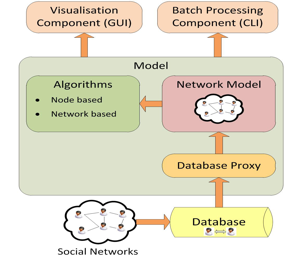
\includegraphics[width=0.4\linewidth]{img/previous_review_system_diagram.png}
	\caption{Figure}
	\label{fig:previous-review-system-diagram}
\end{figure}

As we can see by the design model above, the software was developed using a modular approach with claims of a high degree of extensibility to the existing tool. As C\# .net was used as the base programming language the resulting GUI is of an extremely high standard, with a professional presentation and feel when using it. A criticism however is although the resulting software developed has an extremely well presentable front end, the disadvantage of using a Windows based development environment and programming language is that the software is not transferable between different operating systems. The unfortunate issue with this is that it means the software cannot be run on a Linux or mac based environment. 

 The original design conceived had the algorithms module as a single module with no separation of the type of algorithm to be run or implemented. This was changed in the final design as shown above, so as to provide a greater degree of flexibility for potential researchers using the tool. 

We intend to use the graphical user interface (GUI) in such a way that the interface is essentially a standalone client program. It should be able to access and transmit data and instructions from the client machine to a cluster of machines at the department with the software becoming a lightweight visualisation tool for different social networks or so that it could serve as a dual purpose tool, able to connect and control a cluster of machines or run independently on a single system (e.g. retain all current functionality but incorporate the functionality of a distributed system). The reason for the further development of the previous group's interface is that because the overall look and feel of the GUI is of such a high standard it would be logical to adapt it to the requirements of this project. The database schema is sound and proven to be extremely versatile with the use of Boyce-Codd normal form to reduce data redundancy. This database schema, should the current interface be user-able, is again, another highly desirable  feature of the previous group's work as the ability to switch between a continuous or discrete dataset is implemented extremely well and therefore would allow us to perform research on different types of data such as real time twitter analysis or a batch of data.

There are a few issues to note with this project that have been identified after careful consideration of the requirements of the current project. The main issue that has been identified is the lack of testing in terms of scalability. While the report produced for the social network analysis tool clearly and accurately identifies problems and errors that could arise from use of the tool such as lack of tape (.i.e. the tape that is played when a user plays the message interaction is empty and therefore would throw an error), node properties incorrect or other errors, there were no reports of scalability testing. This could be perceived to be a serious flaw with the tool as it can clearly been seen in the results of research experiments conducted that the tool may have only been tested up to a total of 7000 nodes. While this is quite a large number, we intend to extend the tools ability to incorporate a large amount of twitter data. This form of data consists mostly of a large number of small clusters with a few edges linking clusters together. With nearly 500 million users on twitter and approximately 250 million active users \cite{alltwitter}, the ability to visualise the network along with its associated temporal data is extremely desirable and with many claims throughout the report as to the ability of the tool to handle large amounts of data, it is a concern that the interface we intend to extend with simple object access protocol (SOAP) functionality could not be suitable for the size of graphs we wish to analyse. However, as the tool can be run in CLI mode (batch processing mode without the GUI), the claims of large data processing could in fact be true, however, as we intend to push the computational side of the tool onto a cluster for greater processing power and to achieve a distributed system our main concern with the previous tool is that the interface may not be scalable in terms of graph visualisation.

Another concern is the dependencies structure associated with the design and implementation of the previous tool. As we are only interested in the GUI, it appears substantial changes would need to be made to the tool in order to separate the GUI from the rest of the tool as it is dependant on nearly every other module within the tool. 

While it is clear that the SNA tool was developed to an extremely high standard, the concerns with the previous work in relation to our own is the potential issues with scalability and modular dependency.

There are however, extremely useful sections of the final report produced by the previous group that will in fact prove very useful. For example, they highlight in great detail the operations and possibilities associated with the tool and its database proxy API's developed. This extremely large quantity of high quality specification regarding modules such as the database proxy and the database schema, should prove useful in attempts to dissect the tools structure and code. 
Overall the previous groups work was of a very high standard and the only criticisms that can be put forward apply to issues that they would naturally, given the specification of the SNAT project, not have tested for.

% \chapter{Problem Definition}

\section{Blah}
% \subsection{MapReduce}
MapReduce is a programming framework designed to simply processing data on large clusters \cite{mapreduce}. MapReduce works by the user supplying two functions, Map and Reduce, which operate in parallel on the data set provided. The Map function processes data from key/value pairs into an intermediate set of key/value pairs, before the Reduce function processes this intermediate set into final key/value pairs.

\lstset{language=C++,caption={Calculating the frequency of words in files using MapReduce \cite{mapreduce}},label=lst:mapreduceexample,tabsize=2,breaklines=true,breakatwhitespace=true,frame=single}
\begin{lstlisting}[float]
map(String key, String value):
	// key: document name
	// value: document contents
	for each word w in value:
		EmitIntermediate(w, ``1'');
		
reduce(String key, Iterator values):
	// key: a word
	// values: a list of counts
	int result = 0;
	for each v in values:
		result += ParseInt(v);
	Emit(AsString(result));	
\end{lstlisting}

Listing \ref{lst:mapreduceexample} is an example MapReduce program which counts the frequency of words within a selection of documents stored on a system. The Map function reads each word, \emph{w}, and emits the word as key/value pair \verb/(w, ``1'')/ to signify that there is an occurrence of \emph{w} at that position. The Reduce function sums together the value each of these emitted key/value pairs, where the key is the same, and emits the sum for each word.

Whilst the example given in Listing \ref{lst:mapreduceexample} uses Strings for the input and output for both of the Map and Reduce functions, it is not necessarily the case that all Map and Reduce functions operate in this way. \cite{mapreduce} explains that the types used by both are linked, as shown by:

\begin{verbatim}
map     (k1, v1)        -> list(k2, v2)
reduce  (k2, list(v2))  -> list(v2)
\end{verbatim}

This states the input keys and values are from a different domain to the output keys and values, which also means that the types used can differ.

MapReduce operates in two phases: The Map phase and the Reduce phase. Initially, the input data is split into small chunks to be assigned to the map tasks. A single map task is designated the master, with the remaining tasks designated as workers. The master assigns each map task a chunk of the input data to process, and once this has been processed, it is assigned more until all the input data has been processed. Once data from a map task has been processed, available reduce tasks then process this into the output data from the MapReduce program.

The MapReduce framework is highly fault tolerant, and is able to cope with multiple worker failure and failure of the master program as well. Each worker is required to periodically communicate with the master, and if no communication is received, then the worker is marked as failed, and its work is redistributed back out to be processed again. In case of the master failing, checkpoints are made and the MapReduce program can restart from the last checkpoint recorded.

\subsubsection{Google File System}
The Google File System, GFS, provides the distributed file system which MapReduce operates with \cite{mapreduce}, but was developed outside of MapReduce to address issues found with previous distributed file systems \cite{gfs}.

The GFS was designed to meet three major points identified with existing distributed file systems \cite{gfs}:
\begin{enumerate}
	\item Component failures are the norm, rather than the exception
	\item Files are huge by traditional standards
	\item Files are mutated by appending new data
\end{enumerate}

As hardware failures are common, the design of the GFS incorporates this, and the system is monitoring itself continually to detect, tolerate, and recover promptly from component failures on a routine basis \cite{gfs}. In addition to this, the system used by Google makes use of inexpensive hardware due to the frequent failures experienced, and as such is a more cost-effective solution than using more expensive tailored hardware.

A GFS cluster is split into a single $master$ and multiple $chunkservers$ and is accessed by multiple $clients$ \cite{gfs}. Files stored in the GFS are split into chunks, which are stored across the cluster on the hard disks located on each chunkserver. By default, each chunk is replicated in the file system three times for reliability of access to data within file system.

Files are stored into the GFS in chunks of size 64MB. This size was chosen to reduce the need to interact with master to find the location of chunks to read data from, and write data to. The larger chunk size also reduces the quantity of metadata stored on the master, which increases the performance of the master as the metadata can be stored in memory, reducing lookup times \cite{gfs}.

The master node maintains the metadata for the file system. This includes the locations of chunks across the file system, and which chunks compose the files stored. The master node communicates with each chunkserver frequently, and if it does not receive a response, the chunkserver is deemed to have failed and any chunks which are then under replicated in the file system are re-replicated to ensure that the minimum number of replications for each chunk are observed.

\subsection{Hadoop}
Hadoop\footnote{\url{http://hadoop.apache.org/}} is framework for performing
distributed computing. It is a free implementation of the MapReduce framework
developed at Google, and is also a top-level project hosted by Apache.

Hadoop has diversified itself from its conception, and is now composed of three
subprojects, Hadoop Common, Haddop Distributed File System, and Hadoop
MapReduce. Hadoop Common providse common utilities which support the other
Hadoop subprojects. The Hadoop Distributed File System is described in more
detail in Section \ref{sec:hdfs}

Hadoop MapReduce is the subproject by which Hadoop itself more known for. It
provides functionality similar to the MapReduce framework developed by Google,
where there exists a $Map$ and a $Reduce$ function which process data across a
cluster.

\subsubsection{Hadoop Distributed File System}
\label{sec:hdfs}
Hadoop also provides a the Hadoop Distributed File System, HDFS. The HDFS is a free implementation of the Google File System, and is designed to be used with Hadoop itself, though can also be used a distributed file system by itself \cite{hdfs}.

The HDFS operates in a similar approach to the operation of Hadoop and the Google File System. There exists a master node, called the NameNode, and many slave nodes, called DataNodes. The NameNode co-ordinates the access of files stored in the HDFS, and also manages the file system namespace. There is usually a DataNode present on each physical node within the cluster. It is the DataNode which control the storage of files on the storage system present on the node, and also controls the reading and writing of files to the HDFS from a user.

The HDFS ensures data integrity through replication of data across different nodes within the cluster. A replication factor is set for the cluster, generally at least 3, which causes all data within the HDFS to be replicated at least that many times. Data within the HDFS is split into blocks, with a large file being represented by many smaller blocks, and it is these blocks which are replicated across the HDFS.

In case of a problem with the HDFS, such as a partial network failure, or hard disk failure, each DataNode is required to periodically message the NameNode which contains a report on all data blocks stored by that DataNode. If there is a failure of some kind, then the NameNode either receives an incomplete message or no message at all. This informs the NameNode that there is a problem with the HDFS and takes appropriate action, including re-replicating the lost data from other DataNodes to new DataNodes.

The HDFS also provides another service called the SecondaryNameNode. The SecondaryNameNode is not a direct failover service to the NameNode. Instead, the SecondaryNameNode takes periodic checkpoints of the state of the NameNode, so that in case of the NameNode failing, a recent copy of the state of the HDFS can be loaded when the NameNode is restarted, which should result in minimal problems with resuming the HDFS.


\chapter{Motivation}

\section{Why Is This Important?}
Crimes are frequently committed by a network of individuals, be they loose-knit,
tight-knit, grassroots clusters or hierarchical supply chains. Aspects of the
relationships and power structures that compose these networks are betrayed in
the resulting address books and digital social networks, which the police can
frequently gain access to. However, this information has been distorted, almost
flattened; a deep relationship may appear as a series of unrelated entries in an
addressbook. While direct detective-work is invaluable for making these
connections, the ever-increasing quantity of data to be processed is rendering
this approach less effective. By modelling these networks as graphs, and
through the application of various algorithms, we can attempt to recover some of
this `lost' data. This will provide information about both individual users and
the overall network; cluster identification may detect distinct groups within a
single network and the influence and centrality of individual people can
likewise be calculated. At its simplest this information could help inform
decisions on which people the police should focus their resources on
apprehending, and where in the network to introduce undercover agents to
maximise their influence. 

\subsection{Scale}
As a consequence of the computational complexity of these algorithms, existing tools have
serious scalability issues. The advent of social networking sites has led to
sprawling networks with vast quantities of low-grade information that needs to
be heavily processed to extract anything of value. We have tackled this by
distributing the workload across clusters. Clusters are networks of computers
typically built with commodity-grade components, rendering them cheap and
scalable relative to traditional supercomputers.

\subsection{Relevance}
We chose to use publicly available data from the `microblogging' site Twitter, 
as we lacked access to any police datasets. Twitter is used by two groups the police
are interested in; the `English Defence League' (EDL) and `Unite Against Facism'
(UAF). Previous projects used Enron's emails. Times have changed since then;
emails only make up a fraction of a user's interactions and social networks have
a far higher degree. We demonstrate these techniques on modern, relevant
networks, exploiting the poor operational security exhibited our targets.


\subsection{Alternative Applications: Marketing}
Modelling influence manipulation and the like is also a core requirement of
`viral' marketing; marketers want to choose the ideal starting point in a
network to achieve maximum saturation. At its purest, the website
Sponsored Tweets\footnote{\url{http://sponsoredtweets.com}} allows advertisers to pay a set amount for a tweet from a particular user and influence propagation can be used to inform decisions
about whether a well-connected root is worth the money. 

\subsection{Alternative applications: Persona Management}
This won't just aid manual infiltration by undercover agents; once it is
automated to a suitable degree it may be combined with `persona management
systems'; software that enables a single operator to control large numbers of
fake online identities, massively increasing their voice and influence over
discussions \cite{personaPatent}. Manual identification of influence relationships simply doesn't
scale to this level. Figure \ref{fig:persona_management_workflow} shows an
example persona management flow.


\begin{figure}[htbp]
    \centering
    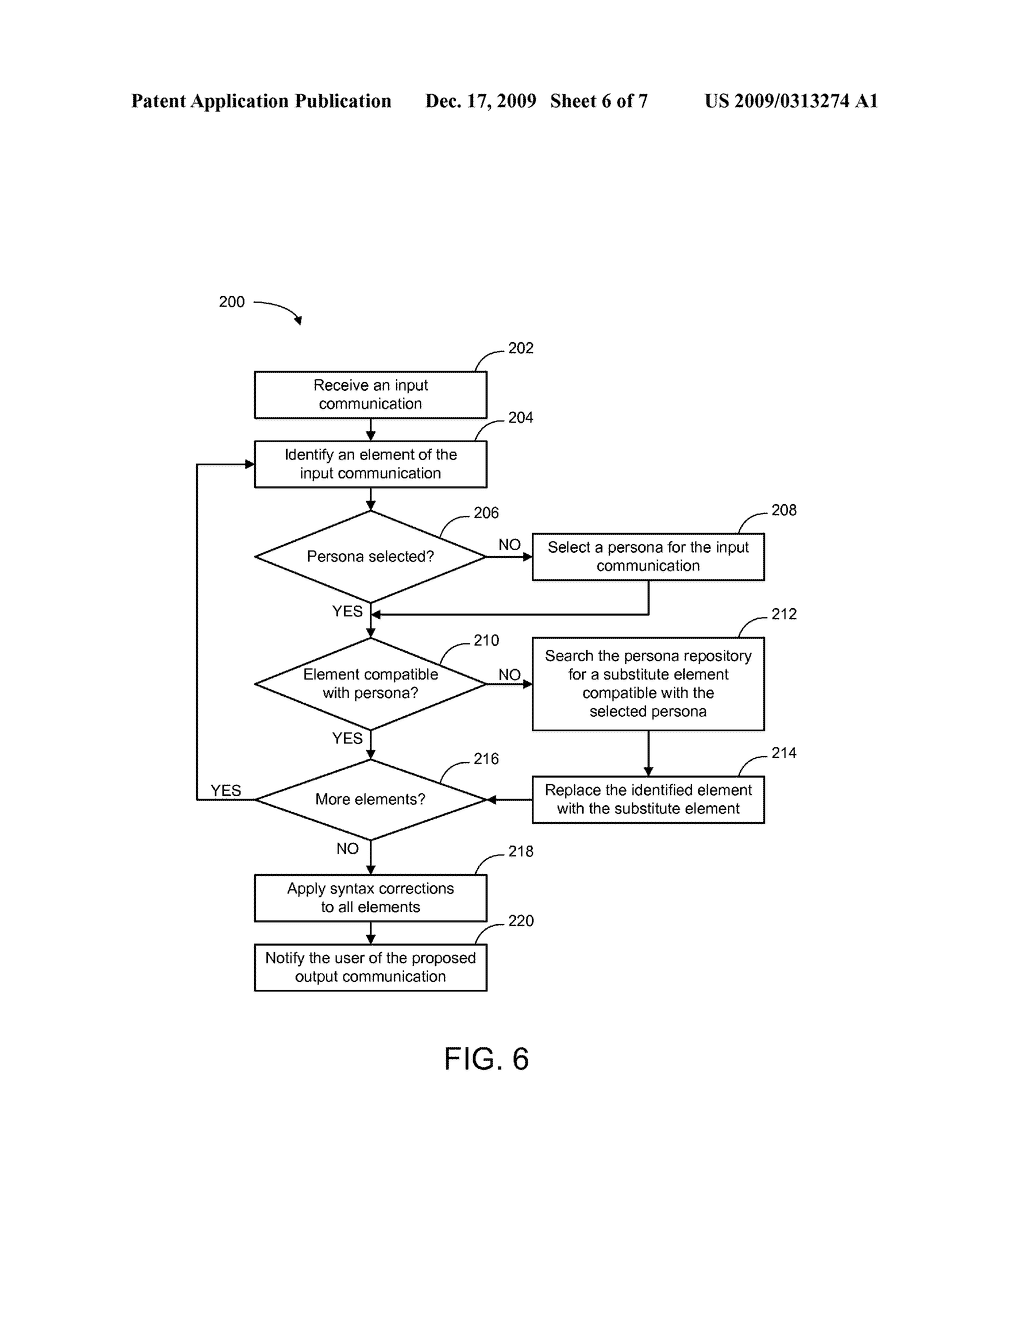
\includegraphics[width=0.7\linewidth]{img/persona_management_flow.png}
    \caption{Persona Management}
    \label{fig:persona_management_workflow}
\end{figure}



% \subsection{MapReduce}
MapReduce is a programming framework designed to simply processing data on large clusters \cite{mapreduce}. MapReduce works by the user supplying two functions, Map and Reduce, which operate in parallel on the data set provided. The Map function processes data from key/value pairs into an intermediate set of key/value pairs, before the Reduce function processes this intermediate set into final key/value pairs.

\lstset{language=C++,caption={Calculating the frequency of words in files using MapReduce \cite{mapreduce}},label=lst:mapreduceexample,tabsize=2,breaklines=true,breakatwhitespace=true,frame=single}
\begin{lstlisting}[float]
map(String key, String value):
	// key: document name
	// value: document contents
	for each word w in value:
		EmitIntermediate(w, ``1'');
		
reduce(String key, Iterator values):
	// key: a word
	// values: a list of counts
	int result = 0;
	for each v in values:
		result += ParseInt(v);
	Emit(AsString(result));	
\end{lstlisting}

Listing \ref{lst:mapreduceexample} is an example MapReduce program which counts the frequency of words within a selection of documents stored on a system. The Map function reads each word, \emph{w}, and emits the word as key/value pair \verb/(w, ``1'')/ to signify that there is an occurrence of \emph{w} at that position. The Reduce function sums together the value each of these emitted key/value pairs, where the key is the same, and emits the sum for each word.

Whilst the example given in Listing \ref{lst:mapreduceexample} uses Strings for the input and output for both of the Map and Reduce functions, it is not necessarily the case that all Map and Reduce functions operate in this way. \cite{mapreduce} explains that the types used by both are linked, as shown by:

\begin{verbatim}
map     (k1, v1)        -> list(k2, v2)
reduce  (k2, list(v2))  -> list(v2)
\end{verbatim}

This states the input keys and values are from a different domain to the output keys and values, which also means that the types used can differ.

MapReduce operates in two phases: The Map phase and the Reduce phase. Initially, the input data is split into small chunks to be assigned to the map tasks. A single map task is designated the master, with the remaining tasks designated as workers. The master assigns each map task a chunk of the input data to process, and once this has been processed, it is assigned more until all the input data has been processed. Once data from a map task has been processed, available reduce tasks then process this into the output data from the MapReduce program.

The MapReduce framework is highly fault tolerant, and is able to cope with multiple worker failure and failure of the master program as well. Each worker is required to periodically communicate with the master, and if no communication is received, then the worker is marked as failed, and its work is redistributed back out to be processed again. In case of the master failing, checkpoints are made and the MapReduce program can restart from the last checkpoint recorded.

\subsubsection{Google File System}
The Google File System, GFS, provides the distributed file system which MapReduce operates with \cite{mapreduce}, but was developed outside of MapReduce to address issues found with previous distributed file systems \cite{gfs}.

The GFS was designed to meet three major points identified with existing distributed file systems \cite{gfs}:
\begin{enumerate}
	\item Component failures are the norm, rather than the exception
	\item Files are huge by traditional standards
	\item Files are mutated by appending new data
\end{enumerate}

As hardware failures are common, the design of the GFS incorporates this, and the system is monitoring itself continually to detect, tolerate, and recover promptly from component failures on a routine basis \cite{gfs}. In addition to this, the system used by Google makes use of inexpensive hardware due to the frequent failures experienced, and as such is a more cost-effective solution than using more expensive tailored hardware.

A GFS cluster is split into a single $master$ and multiple $chunkservers$ and is accessed by multiple $clients$ \cite{gfs}. Files stored in the GFS are split into chunks, which are stored across the cluster on the hard disks located on each chunkserver. By default, each chunk is replicated in the file system three times for reliability of access to data within file system.

Files are stored into the GFS in chunks of size 64MB. This size was chosen to reduce the need to interact with master to find the location of chunks to read data from, and write data to. The larger chunk size also reduces the quantity of metadata stored on the master, which increases the performance of the master as the metadata can be stored in memory, reducing lookup times \cite{gfs}.

The master node maintains the metadata for the file system. This includes the locations of chunks across the file system, and which chunks compose the files stored. The master node communicates with each chunkserver frequently, and if it does not receive a response, the chunkserver is deemed to have failed and any chunks which are then under replicated in the file system are re-replicated to ensure that the minimum number of replications for each chunk are observed.

\subsection{Hadoop}
Hadoop\footnote{\url{http://hadoop.apache.org/}} is framework for performing
distributed computing. It is a free implementation of the MapReduce framework
developed at Google, and is also a top-level project hosted by Apache.

Hadoop has diversified itself from its conception, and is now composed of three
subprojects, Hadoop Common, Haddop Distributed File System, and Hadoop
MapReduce. Hadoop Common providse common utilities which support the other
Hadoop subprojects. The Hadoop Distributed File System is described in more
detail in Section \ref{sec:hdfs}

Hadoop MapReduce is the subproject by which Hadoop itself more known for. It
provides functionality similar to the MapReduce framework developed by Google,
where there exists a $Map$ and a $Reduce$ function which process data across a
cluster.

\subsubsection{Hadoop Distributed File System}
\label{sec:hdfs}
Hadoop also provides a the Hadoop Distributed File System, HDFS. The HDFS is a free implementation of the Google File System, and is designed to be used with Hadoop itself, though can also be used a distributed file system by itself \cite{hdfs}.

The HDFS operates in a similar approach to the operation of Hadoop and the Google File System. There exists a master node, called the NameNode, and many slave nodes, called DataNodes. The NameNode co-ordinates the access of files stored in the HDFS, and also manages the file system namespace. There is usually a DataNode present on each physical node within the cluster. It is the DataNode which control the storage of files on the storage system present on the node, and also controls the reading and writing of files to the HDFS from a user.

The HDFS ensures data integrity through replication of data across different nodes within the cluster. A replication factor is set for the cluster, generally at least 3, which causes all data within the HDFS to be replicated at least that many times. Data within the HDFS is split into blocks, with a large file being represented by many smaller blocks, and it is these blocks which are replicated across the HDFS.

In case of a problem with the HDFS, such as a partial network failure, or hard disk failure, each DataNode is required to periodically message the NameNode which contains a report on all data blocks stored by that DataNode. If there is a failure of some kind, then the NameNode either receives an incomplete message or no message at all. This informs the NameNode that there is a problem with the HDFS and takes appropriate action, including re-replicating the lost data from other DataNodes to new DataNodes.

The HDFS also provides another service called the SecondaryNameNode. The SecondaryNameNode is not a direct failover service to the NameNode. Instead, the SecondaryNameNode takes periodic checkpoints of the state of the NameNode, so that in case of the NameNode failing, a recent copy of the state of the HDFS can be loaded when the NameNode is restarted, which should result in minimal problems with resuming the HDFS.


\chapter{Research}
This chapter discusses 

The main areas of interest are community detection and how information spreads throughout a social network. 

% Since we have a few distinct sections on this area, I think it's a good idea to split this into multiple smaller files as well

\section{Social Network Analysis}
\subsection{Community Detection}
An important aspect of social network analysis is the detection of communities within a graph. The identifying of communities within a social network can help to identify group dynamics of the network. 

A famous example of this is the friendship network within Zachary's karate club \cite{zachary77}, which subsequently split into the two groups shown in Figure \ref{fig:karate}. The identification of two clusters, which cleanly divided the network into the two groups the karate club actually split into, shows the usefulness of being able to identify connections between groups of highly interlinked individuals.

\begin{figure}%
\centering
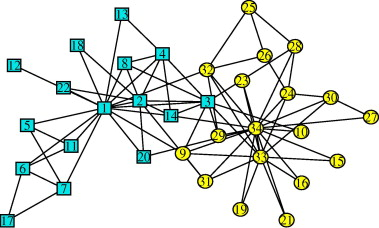
\includegraphics[width=0.5\columnwidth]{./img/karate}%
\caption{Clusters found within Zachary's karate club \cite{zachary77,comellas10}}%
\label{fig:karate}%
\end{figure}

\subsubsection{Clustering}
Within social networks, there are distinct regions of vertices with many connections passing between them, and a much smaller number connected to other vertices outside of this region. These regions are termed as \emph{clusters}.

Social networks are a prime example of this. A person tends to have groups of friends distinct from each other, and friends within these groups are also friends of each other. Figure \ref{fig:socialnetwork} is a social network constructed from data regarding mutual friends of a person. Within this Figure, it can clearly be seen that there exists five distinct regions of mutual friends, with very few links between these regions. These regions are the clusters described above.

With data presented in this manner, it is clear to an observer where these clusters exist, and how many distinct clusters there are. \cite{girvan02} presents an approach to identifying communities within a graph.

\begin{figure}[htbp]
\centering
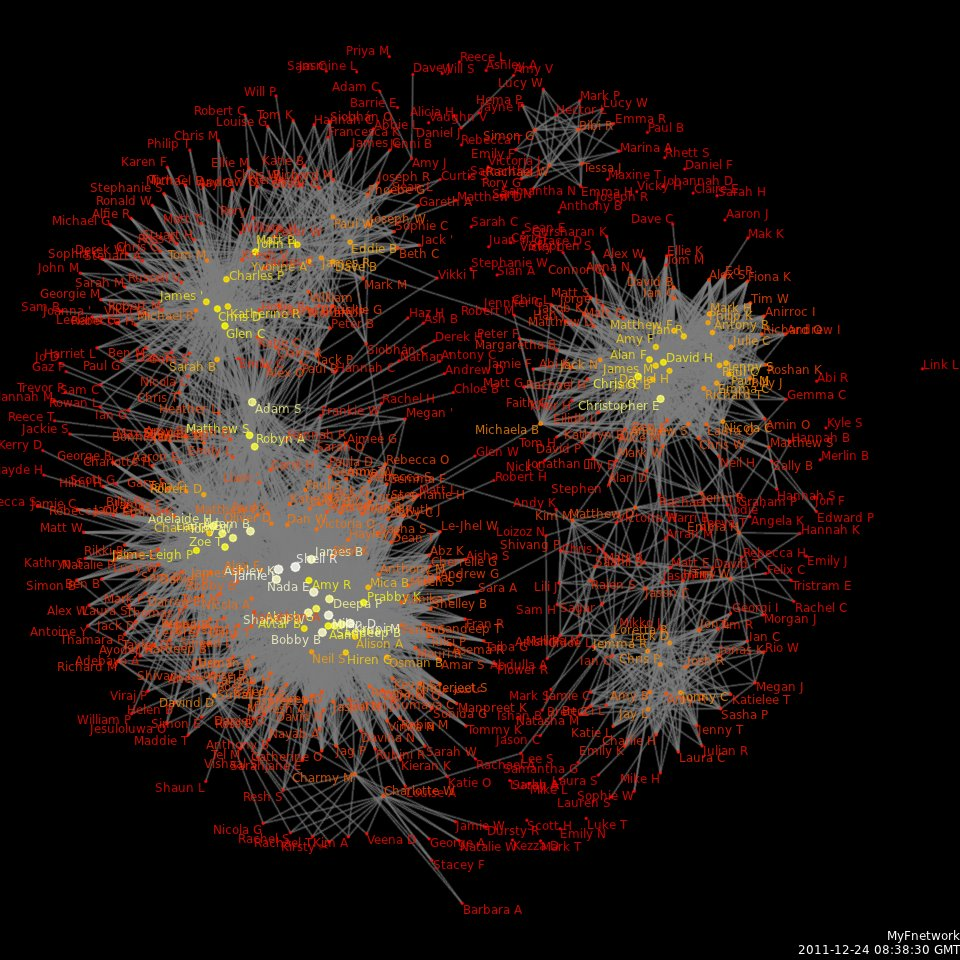
\includegraphics[width=0.5\textwidth]{./img/socialnetwork.png}
\caption{Social Network constructed from Facebook friends using the myFnetwork app}
\label{fig:socialnetwork}
\end{figure}

\subsubsection{Partitioning}
Partitioning of a graph differs from clustering slightly. To partition a graph, we first must know the number of partitions we wish to make, and also the size of each of these partitions. Clustering does not need to know this information as the clusters are produced by the algorithms performing the clustering. Partitioning is related to clustering as it splits the input graph into distinct smaller subgraphs of highly connected vertices, with the subgraphs representing communities within the original graph.

The process of graph partitioning is to divide a graph into smaller parts, such that the number of connections between these smaller parts is as few as possible. The partitions produced are non-overlapping, of a given size, and of a given number.

Graph partitioning is known to be a difficult and complex problem to solve. For simplicity, assume that we are to partition a graph into two partitions. To naively \emph{brute force} all permutations to find the ``best'' partition, which minimises the number of connections between the two partitions, soon becomes unfeasible for anything but the smallest graphs, due to the number of ways of partitioning \emph{n} verticies into two groups \emph{$n_1$} and \emph{$n_2$}. This is $\frac{n!}{n_1!n_2!}$ permutations, and with application of Stirling's formula, can we rewritten as \cite{newman10}:

\begin{equation}
\frac{n!}{n_1!n_2!} \simeq \frac{\sqrt{2\pi n}(n/e)^n}{\sqrt{2\pi n_1}(n_1/e)^{n_1} \sqrt{2\pi n_2}(n_2/e)^{n_2}} = \frac{n^{n+1/2}}{n_1^{n_1+1/2} n_2^{n_2+1/2}} 
\label{eq:partioning1}
\end{equation}

Which, if our two partitions $n_1$ and $n_2$ are equal in size, then the number of permutations of the partition is \cite{newman10}:

\begin{equation}
\frac{n^{n+1/2}}{(n.2)^{n+1}} = \frac{2^{n+1}}{\sqrt{n}}
\label{eq:}
\end{equation}

This shows that running time of the \emph{brute force} algorithm to find all permutations grows exponentially with the size of the input graph.

\citeauthor{kernighan70} proposed an algorithm to solve the partitioning of a graph into two sections \cite{kernighan70}. Initially, the graph is split into two partitions, \emph{A} and \emph{B}. For each pair of vertices (\emph{i, j}) such that $i \in A$ and $j \in B$, the algorithm finds the pair which reduces the number of connections between \emph{A} and \emph{B} the most (see Figure \ref{fig:kernighanlin1}), and swap them (Figure \ref{fig:kernighanlin2}). If there is no pair which reduces the number of connections between the two partitions, then the pair which increases the number of connections by the smallest amount are swapped. This is then repeated until vertices within one partition have been swapped, with the condition that once a vertex has been swapped, it cannot be swapped again. Following this, each state the graph was in after a swap is revisited, with the state with the minimum number of connections between \emph{A} and \emph{B} is minimal. These steps are then repeated until \emph{A} and \emph{B} do not change between rounds. The algorithm has been shown to run in $O(n^2\: log\: n)$ time \cite{kernighan70}, which is marked improvement over the \emph{brute force} $O(2^n)$, but still remains slow and unsuitable for graphs with a over a few thousand vertices \cite{newman10}.

\begin{figure}[htbp]
  \centering
  \subfloat[Original network]{\label{fig:kernighanlin1}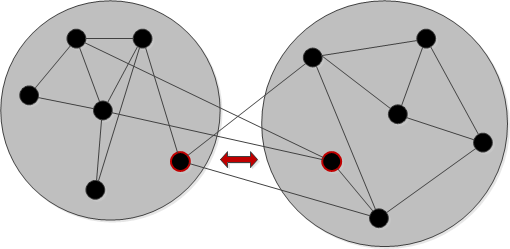
\includegraphics[width=0.3\textwidth]{./img/kernighanlin1}}
  ~ 
  \subfloat[The same network after interchange of two vertices]{\label{fig:kernighanlin2}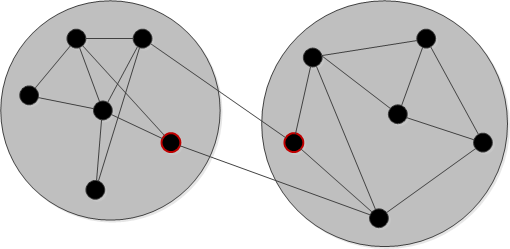
\includegraphics[width=0.3\textwidth]{./img/kernighanlin2}}
  ~ 
  \caption{The Kernighan-Lin algorithm \cite{newman10}}
  \label{fig:kernighanlin}
\end{figure}

Figure \ref{fig:kernighanlin} shows the effect of the Kernigham-Lin algorithm on the original network (Figure \ref{fig:kernighanlin1}). The two vertices highlighted with red reduce the number of connections between the two groups the most, so are swapped. This swap is also the best swap which happens during this iteration of the algorithm, so the network in Figure \ref{fig:kernighanlin2} is selected as the initial network for the next iteration. As no vertex swapping can improve on this, and as such this network is the best network for the next iteration, this network is the solution from the algorithm and the algorithm terminates.

To split a graph into more than two partitions, repeated application of partitioning the subgraphs produced from previous partitioning is applied.

There exist other algorithms to partition graphs, notably spectral algorithms \cite{pothen90,fiedler73}, which make use of properties of the matrix which can be used to define a graph. These spectral algorithms are a lot more complex in the operations needed to execute them, however they operate in $O(n^2)$ time, which is an order $n$ faster than the Kernighan-Lin algorithm \cite{newman10}. It is also noted that spectral algorithms do not necessarily give the best partition, with the partitions produced being of the rough general shape but not quite as good as other algorithms \cite{newman10}.

\subsubsection{\emph{k}-Cliques}
The term \emph{clique} is introduced by \citeauthor{luce49} in \cite{luce49} to describe a subgraph which consists of at least three vertices, each of which are fully connected with each other. From a social network perspective, this translates to saying that for each person in the clique, all of their friends  within the clique are friends of each other as well.

A \emph{k}-clique is defined as a clique which has size \emph{k}. A \emph{maximal clique} is a clique to which no more vertices can be added without violating the conditions of a clique, and the maximum clique is a clique within a graph which contains the largest number of vertices. A 3-clique is also known as a triangle, due to the shape of the graph they are normally represented as (Figure \ref{fig:3clique}).

\begin{figure}[htbp]
\centering
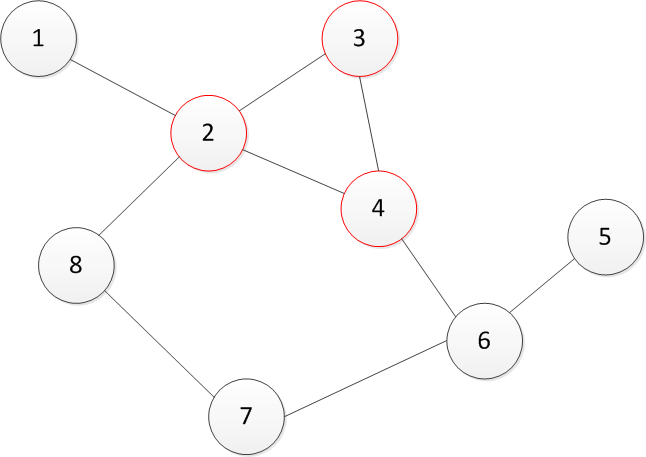
\includegraphics[width=0.5\textwidth]{./img/clique.png}
\caption{Graph highlighting a 3-clique}
\label{fig:clique}
\end{figure}

Figure \ref{fig:clique} shows an example graph highlighting a 3-clique. It has one maximum clique \{2,3,4\} which is highlighted in red, and six other maximal cliques \{1,2\}, \{2,8\}, \{4,6\}, \{5,6\}, \{6,7\}, \{7,8\}.

\begin{figure}
  \centering
  \subfloat[3-clique]{\label{fig:3clique}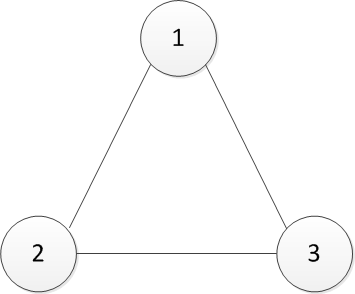
\includegraphics[width=0.3\textwidth]{./img/3-clique}} ~ \subfloat[4-clique]{\label{fig:4clique}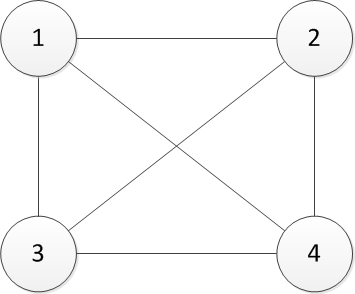
\includegraphics[width=0.3\textwidth]{./img/4-clique}} ~ \subfloat[5-clique]{\label{fig:5clique}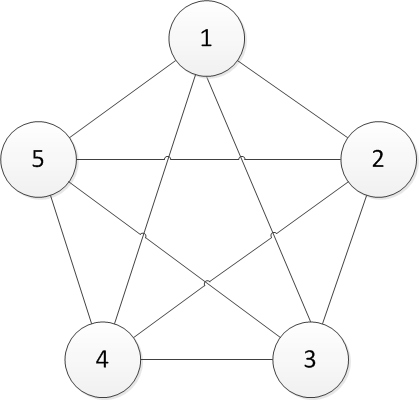
\includegraphics[width=0.3\textwidth]{./img/5-clique}}
  \caption{\emph{k}-cliques}
  \label{fig:cliques}
\end{figure}

Identifying cliques, and solving problems involving cliques as been shown to be computationally hard \cite{bomze99, trusses}. Cliques are either too common, with cliques of only a few members are frequently too numerous to be helpful, or too rare, with large cliques too limiting to be of use \cite{trusses}. Also, computation of identifying cliques scales worse than any polynomial of the problem size, making the process unfeasible for large graphs \cite{trusses, bron72}.

There have been numerous generalisations of the clique construct to improve usefulness of the clique through relaxation of some of the properties of the clique. These include the \emph{n}-clique \cite{luce50}, \emph{n}-clan \cite{alba73} and \emph{n}-club \cite{mokken79}. However these new constructs do not solve the issues of identifying cliques, and remain hard to compute and produce too many results.

\subsubsection{\emph{k}-Trusses}
Following from relaxing properties of the clique, \citeauthor{trusses} in \cite{trusses} introduces a new construct called a truss. A \emph{k}-truss is a subgraph where an edge between two vertices, A and B, exists if at least \emph{k-2} other vertices are connected to both of A and B. The \emph{k}-truss has similar definitions to the clique. A maximal \emph{k}-truss is a \emph{k}-truss that is not a proper subgraph of another \emph{k}-truss.

\begin{figure}[htbp]
\centering
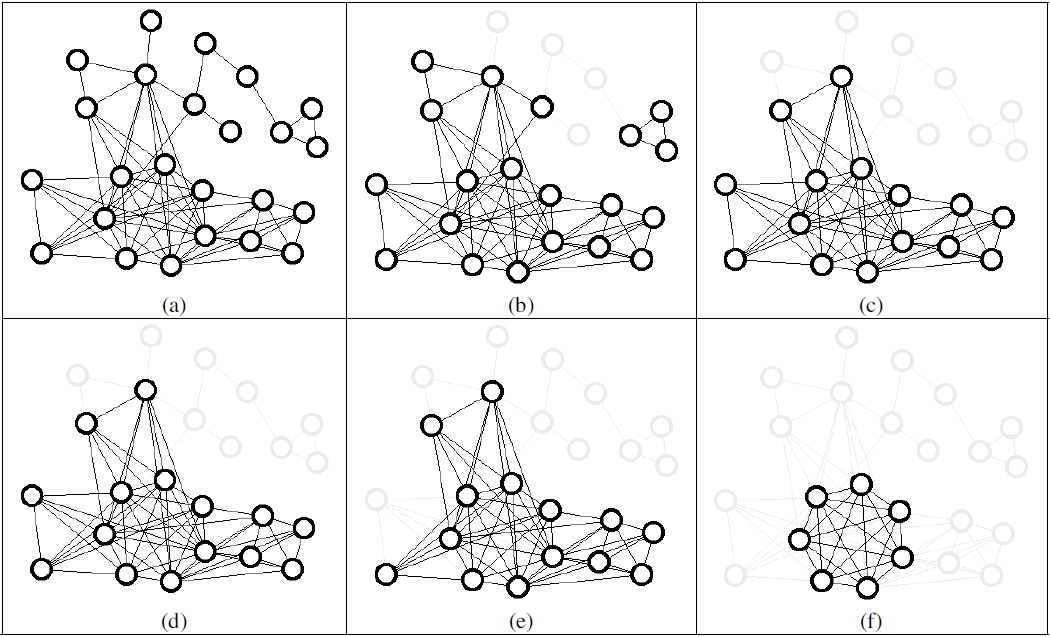
\includegraphics[width=0.9\textwidth]{./img/trusses.png}
\caption{An Example of Maximal Trusses. (a) original graph, (b) 3-trusses, (c) 4-truss, (d) 5-truss, (e) 6-truss. Note that (c) and (d) are the same. \cite{trusses}}
\label{fig:trusses}
\end{figure}

Figure \ref{fig:trusses} shows an example application of \emph{k}-trusses. Figure \ref{fig:trusses}(a) shows the original graph. Figures \ref{fig:trusses}(b-f) show the \emph{k}-truss for increasing values of \emph{k}. If the same original graph were to be analysed for \emph{k}-cliques for the same values of \emph{k}, more vertices in the graph would have been removed in earlier stages, which would have lost the interesting stage where Figures \ref{fig:trusses}(c) and (d) are identical.

The \emph{k}-truss is also computable in polynomial time to the input graph, which offers a marked improvement on the computation costs of identifying cliques and similar constructs. \cite{trusses} shows that the naive algorithm  for computing maximal \emph{k}-trusses is bounded by $O(n|E|^2 + n)$, where \emph{n} is the number of vertices in the graph, and \emph{|E|} is the number of edges in the graph. A more efficient method is shown to take $O(\Sigma d^2(v))$, where \emph{d(v)} is the degree of a vertex, \emph{v}.

\subsection{Clustering Coefficients}
Clustering coefficients provide a way to measure the amount to which vertices within a graph cluster together. Calculating clustering coefficients requires knowing the number of triangles within the graph.

\subsubsection{Global Clustering Coefficient}
The global clustering coefficient is also known as the transitivity of a network. This is because it is similar to the mathematical property of transitivity. A relation ``$\circ$'' is said to be transitive if $a \circ b$ and $b \circ c$ imply together imply $a \circ c$. An example would be the equality relation, as if $a = b$, and $b = c$ it follows that $a = c$ \cite{newman10}. Within a social network, the transitive relation could be described as \textit{``the friend of my friend is also my friend''}.

A global clustering coefficient of 1 implies a social network where all components are cliques. A global clustering coefficient of 0 implies a social network where there are no mutual friends between any two people.

The global clustering coefficient is defined as:

\begin{equation}
C_G = \frac{3 * number\: of\: triangles}{number\: of\: connected\: triples}
\label{eq:globalcc}
\end{equation}

A connected triple is simply three vertices $uvw$ connected with edges ($u, v$) and ($v, w$); edge ($u, w$) does not need to be present \cite{newman10}. The factor 3 is present because each triangle is composed of three connected triples.

\subsubsection{Local Clustering Coefficient}
A clustering coefficient can also be applied to each vertex within a graph. The local clustering coefficient is the probability that vertices connected to a vertex are themselves also connected to each other.

The local clustering coefficient is defined as:

\begin{equation}
C_L = \frac{number\: of\: triangles\: connected\: to\: vertex\: v}{number\: of\: triples\: centered\: on\: vertex\: v}
\label{eq:localcc}
\end{equation}

Within social network analysis, the local clustering coefficient

\subsubsection{Network Local Clustering Coefficient}
The network local clustering coefficient is simply the mean of all local clustering coefficients within a network. It can be used to show the average level of connectedness between vertices in a network.

\begin{equation}
C_N = \frac{1}{n}\sum_{i=1}^{n} C_i
\label{eq:networkcc}
\end{equation}

$C_i$ represents the local clustering coefficient of the vertex $i$. The result of this calculation is a number between 0 and 1, with 1 meaning all vertices are connected to each other \cite{watts98}.

\subsection{Centrality}
Following from identifying communities within a social network, it is also apparent that establishing the most \emph{central} or \emph{important} person is within a community. This person is most likely going to have a large influence over the members of the community 

\subsubsection{}
\subsection{Influence Propogation}

 Influence propogation algorithms attempt to model the spread of ideas (Rogers 2003), viruses (Anderson and May 1991), word-of-mouth recommendations (Goldenberg, Libai and Muller 2001), viral marketing campaigns (Kempe, Kleinberg and Tardos 2003) or other transmissable entities, through a social network.

Influence propogation algorithms make the following assumptions about the social networks that they model. Social networks are modelled as directed graphs, with nodes representing individuals, and vertices representing relationships between individuals. In most influence propogation models, nodes can be in one of two states: "converted" or "unconverted". At the begin of the simulation, a subset of the nodes will be converted; over time they will convert their unconverted neighbours. There is an assumption of monotonicity, ie, converted nodes do not become unconverted.

 The exact conditions that determine when nodes will change from unconverted to converted depends on the influence propogation model used. There are three main models of transmission used; the independent cascade model, the linear threshold model, and ???

Mention more complicated models, three states etc

\subsubsection{Independent Cascade}
 In the independent cascade model, whenever a node becomes converted, it has one chance to convert each of its neighbours. Every edge (A -> B) is assigned a weight between 0 and 1, which represents the probability that node A can convert node B, or vice versa.

Assume a node n has a set of x neighbours n\_0,n\_1,n\_2...n\_x each with edge weights e\_0,e\_1,e\_2...e+x. When n is converted, each neighbour n\_m has a e\_m chance to become converted.

This can be expressed in pseudocode as follows:

recently-converted-nodes = a queue of the initially converted nodes
while recently-converted-nodes is non-empty {
  node = recently-converted-nodes.next()
  for each neighbour in node.neighbours {
    if rand(0,1) < neighbour.edge-weight {
      neighbour.converted = true
      recently-converted-nodes.enqueue(neighbour)
    }
  }
}

\subsubsection{Linear Threshold}
 In the linear threshold model, every node has a threshold value t. When the number of converted neighbours is greater than t, the node becomes converted. Again, edges can be weighted, in which case the condition for conversion is:

Maths: sum for all neighbours(if neighbour is converted(0,1) * edge weight)

That is, nodes are converted when a threshold of their neighbours are converted. In pseudocode:

do {
  changed-nodes = 0
  for each node in unconverted-nodes {
    neighbour-influence = 0
    for each neighbour in neighbours {
      if neighbour.converted {
        neighbour-influence += neighbour.edge-weight
      }
    }
    if neighbour-influence >= node.threshold {
      node.converted = true
      changed-nodes += 1
    } 
  }
} while changed-nodes > 0

\subsubsection{Decreasing Cascade Model}


\subsubsection{Influence Maximisation Problem}

[Maximizing the Spread of Influence through a Social Network]

[http://arxiv.org/pdf/math/0612046.pdf]

One common use of an influence propogation model is to determine the best subset of nodes, that, if converted at the start of the simulation, will maximise the number of converted nodes at the end of the simulation. More formally, given a fixed budget k, and a function f(S), which takes an initial set of converted nodes and computes the expected final number of converted nodes, find a set of k nodes that maximises f(S).

One practical example would be a viral marketing company that might wish to kickstart their campaign by giving a group of influential bloggers a free trial of their service, and hope that these bloggers would then hopefuly recommend the product to their followers, who would recommend it to their followers, and so on. One strategy for choosing the optimal set of free trial users would be to rank the bloggers by a precomputed influence rating, and then select the top k most influential individuals from the list.

Even if influence of a single node could be computed reliably, this strategy would not generally find the optimum subset. For example, the most influential bloggers might share the same audience, wheras a less popular blogger might have considerable influence amongst a niche audience. In graph theory terms, there may be a short distance between two influential nodes -- they may even share overlapping neighbourhoods -- which means there may be a set of nodes far from the influential pair. These nodes might be more influenced by a node that is less globally influential, but nearer. Obviously, the structure of the graph determines the likelihood of this. For example, graphs with a community structure are more likely to require an influential seed node within each community to achieve maximum influence.

Solving the optimum problem is NP-hard, for both the linear threshold and independent cascade models. This can be shown by reducing the independent cascade maxmisation problem to a special case of the set cover problem, and the linear threshold maximisation problem to a special case of the vertex cover problem.

However, a greedy solution works as an approximation. !he set of nodes chosen by the greedy solution will convert at least 63\% of the nodes converted by the optimum solution. This result can be proved by showing that the function f(S) is monotonic and submodular.

The monotonicity property requires that f(S) increases whenever an element is added to S; ie, f(S+v) >= f(S) for any S, v. Proving this property of f(S) is trivial. The submodularity property can be intuitively thought of as a ``dimininishing returns'' property; if S is a subset of T, the marginal gain from adding an element v to S is at least as high as adding the same element to T. Formally:

f(S+v) - f(S) >= f(T+v) - f(T)

Nemhauser, Wolsey and Fisher showed that a greedy-hill climbing algorithm can be used to find the optimum value of such a submodular function to within a factor of 1/(1-e), or ~63\%. The greedy algorithm works by adding elements to the seed set one at a time, each time choosing the element that provides the largest marginal increase to the value of the function. In the case of influence maximisation, this is the node that adds the greatest number of converted nodes at the end of the simulation.

Of course, this method relies on a fast method of working out the expected number of nodes that will be converted by a seed set. There is currently no simple means of calculating this value, so in practice a Monte Carlo method is used; ie, running several iterations of the model and taking an average of the final number of converted nodes. This is computationally expensive, though some work has been done to improve the performance. [CITE??]

\subsubsection{Adversarial Social Networks}

 There are limitations to the two-state models described above. For example, they cannot represent any scenario where two competing ideas spread through a network. An alternative model for such situations allows nodes to be in one of 3 states; "unconverted", "converted to idea A", or "converted to idea B". In this case, A and B represent opposing beliefs.

The paper [Influence Propagation in Adversarial Social Network—Impact of Space and Time] looks in depth at this situation, and applies it to the spread of radical and counter-radical ideas through the Muslim community.

They observe that the key reason that the standard influence propogation model cannot capture the nature of adverserial networks is as follows. Observe the network described in fig???. Node\_2 is initially converted to idea A, and node\_4 is converted to idea B. All other nodes are unconverted. At some point, node\_9, which is a bottleneck between the two sides of the graph, may be converted to one idea or the other. Once this happens -- assume that it is converted to idea A -- there will be no chance that it will ever be converted to idea B. For that reason, there is no way that idea B can ``pass through'' node\_9 and so no way that nodes 10 to 14 will ever be converted to idea B. The standard influence models have no way to capture this situation.

\begin{figure}[htbp]
\centering
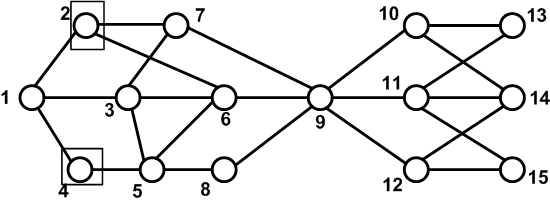
\includegraphics[width=0.5\textwidth]{./img/adversial_network.png}
\caption{Adverserial network}
\label{fig:adverserial_network}
\end{figure}

Other real-life applications of this concept include marketing -- promoting your product while a rival company is promoting a competing product -- or preventing the spread of misinformation. A recent example was the Kony 2012 campaign, a viral video spread by a non-profit activist organisation to highlight the issue of child soldiers in Uganda. The video spread very rapidly via online social networks; however, this soon led to people questioning the aims and methods of the campaigning organisation. This led to a counter-campaign that also spread virally, via social media. (Of course, which party provided misinformation in this scenario depends on individual perceptions).

[Limiting the Spread of Misinformation in Social Networks] looks more in depth at the problem of countering mis-information. They quantify this situation as a ``Multi-Campaign Independent Cascade Model'', where two campains, C and L, spread through a network. Each campaign has an initial seed set of nodes, A\_C/A\_L. As with the independent cascade model, when a node is converted, it has one chance to convert each of its neighbours. The probability that a node n converts its neighbour o is given by p\_C\_n\_o / p\_L\_n\_o, depending on which campaign the node was converted to. Note that in the general case, their may be different probabilities for the two campaigns (representing the situation where one campaign is more ``infectious'' than the other). Unlike in the independent cascade model, when an unconverted node has multiple converted neighbours, the order of ``conversion attempts'' matters; eg, campaign C may succeed in converting a node before campaign L has had the chance to convert it. Their model assumes that one campaign always precedes the other in such situations, ie, that campaign always gets the ``first chance''.

They also used a more specific model, the ``Campaign Oblivious Independent Cascade''. This is a special case of the multi-campaign model, where the conversion probabilities are the same for both campaigns.

They then look at minimising the influence of the opposing campaign, as opposed to maximising their own influence; this problem is referred to as the ``eventual influence limitation problem''. This can also be seen as maximising a function g(S), where S represents the seed set of campaign A (the ``good'' campaign), and g(S) computes the number of ``saved'' nodes -- ie, the number of nodes that were converted to campaign A, but would have been converted to campaign B if A was not present. Even with some simplifying assumptions (campaign B has a seed set consisting of only one node, campaign A has a conversion probability of 1), the problem is still NP-hard.

However, as with the two-state influence models, the function g can be shown to be submodular, and therefore a greedy algorithm can again achieve a performance of 1-(1/e) or ~63\%. This greedy algorithm works similarly to the one used for the influence maximisation problem; ie, iteratively adding to the seed set the node that will provide the best marginal improvement.

Although this is a polynomial-time algorithm, the datasets used for practical social network analysis may be extremely large, making even this algorithm unworkable in practice. Some alternative heuristics are therefore possible. These include the ``degree centrality heuristic'' (ie, choosing the nodes with the most incident edges), the ``early infectees heuristic'' (ie, choosing the nodes that are expected to be infected by the rival campaign early on), and the ``largest infectees heuristic'' (ie, choosing the nodes that are expected to infect the highest number of other nodes). By evaluating these heuristics via Monte Carlo simulations, it can be shown that the largest infectees heuristic is the most effective, approaching the performance of the greedy algorithm. The early infectees heuristic proved to be the least effective approach.




- Influence Maximisation Problem
-- limited budget of initially converted nodes
-- constrained optimisation problem
-- algorithm: non-negative, monotone, submodular
-- greedy algorithm

- attempt to find most influential nodes in a network

Cascading influence in blogs
http://cs.stanford.edu/people/jure/pubs/blogs-sdm07.pdf
- links between blogs
- 45k blogs and 2.2m posts
- is it bursty and/or periodic? does interest die off linearly or exponentially?
- popularity drops off in a power law
- size distribution of cascades follows a Zipfian distribution
- human networks tend to follow a power law distribution
- analyses cascade shapes

What stops social epidemics?
- existence of ``epidemic threshold'', critical value of transmissability
- large degree of heterogenity speeds up epidemics (Superspreading and the effect of individual variation on disease emergence.)

Digg
- spread of interest (votes) for a story through a users' friends
- not epidemic, why? network structure, 
- no increased chance to convert with multiple converted neighbours (friend saturation model)
- scale free number of fans
- only one epidemic story, michael jackson
- decreasing cascade model

A simple model of global cascades on
random networks
``These phenomena are all examples of what economists call
information cascades (ref. 4; but which are herein called simply
cascades), during which individuals in a population exhibit
herd-like behavior because they are making decisions based on
the actions of other individuals rather than relying on their own
information about the problem.''


\section{Emergent Behaviour}

The purpose of this component of the project is to observe and
describe how networks converge and to look at how robust these
networks are in the presence of infiltrators.  More specifically,
we will be looking at networks which use a tag-based approach to
cooperation and the infiltrators will be self-interested agents
which do not follow the social norms of the network.  In our case,
these self-interested agents could be thought of as law-enforcement
individuals.  In general, the presence of self-interested agents
have a negative affect on the cooperation within such a network.
Therefore, we will look at methods to preserve the cooperation rates
in networks where self-interested agents are present.

\subsection{Existing Research}

We are extending the work of Griffiths and Luck (2010) on tag-based
cooperation in a network in the presence of self-interested agents.
This work employs an image-scoring mechanism, network rewiring, and
a learning-based approach to evolution.

The work by Griffiths and Luck extends previous work on tag-based
cooperation, especially Riolo, Cohen, and Axelrod (2001); and Hales
and Edmonds (?).

\subsection{RCA Tag-based Cooperation}

Tag-based cooperation was introduced (Riolo, Cohen and Axelrod,
2001) to observe the nature and method that cooperation in a network
emerges.

The cooperation approach described by RCA takes place in a population
of agents.  Each agent is assigned a single tag and a single tolerance
value.  Both the tag and tolerance are selected randomly from a
uniform distribution between 0 and 1.
The tag is a cultural artefact, a form of a public identifier.
The tolerance is used to determine the willingness of an agent to cooperate.

The approach described by RCA is generational.  Each generation is
divided into two phases: a donation phase and a reproduction phase.
The donation phase occurs first, which allows every agent to perform
a number of donations.  After the donation phase, the reproduction
phase allows agents to reproduce based on their relative success.

During the donation phase, each agent in the population is selected
to make a number of donations.  The number of donations each agent
is selected to make is known as the number of interactions pairings
per generation, P.  When an agent has been selected for donation,
they pick an agent at random to which they have the opportunity to
donate.  In the RCA approach, an agent will donate to the random
agent if the difference between the two agents' tags is less than
the tolerance of the donator.  If an agent chooses to donate, they
will incur a small cost, c, and provide a benefit, b, to the receiving
agent.

\begin{align*}
    |\tau_A - \tau_B| < T_A
\end{align*}

The cooperation of a population of agents is measured by the donation rate in each generation.

Once every agent has been given an opportunity to donate $P$ times,
the reproduction phase takes place.  During the reproduction phase,
each agent reproduces in accordance with their relative success.
The most successful agents produce more offspring than the less
successful agents.  Each agent compares itself to a random agent.
If the agent is less successful than the random agent, then its
offspring derives from the random agent.  If the agent is more
successful than the random agent, then its offspring derives from
iteself.  The offspring takes the tag and tolerance values of the
more successful agent.  There is a small chance that the tag and
tolerance values could be mutated.  If the tag is mutated, the
offspring will receive a new tag taken randomly from the uniform
distribution $\left[0, 1\right]$.  If the tolerance is mutated, a
small amount of gaussian noise with a mean of $0$ is added to the
tolerance value.

Once the donation and reproduction phases for a given generation
have occurred, the process is repeated on the new population.

RCA noted that the donation rate quickly stabilises after around
100 generations.  Occasionally, an agent gets a tolerance value
that is much smaller than the average tolerance as the result of a
mutation.  This mutation allows the agent to become more successful
as they are less likely to donate.  The impact of this reduces the
overall donation rate until the agents converge on the new tag---due
to the reproduction process---at which time the donation rate raises
and stabilises again.

By experimentation, RCA found that with a higher number of interaction
pairings in each generation, the donation rate and average tolerance
increases.  RCA also noted that when the cost of donating became
too high relative to the benefit of receiving a donation, the
donation rate dropped dramatically.  From these results, we will
choose the number of interaction pairings per generation, $P$, to
be at least $3$, the cost of donation to be $0.1$, and the benefit
of receiving a donation to be $1$.

\subsection{Learning-Interpretation of Reproduction}

Hales and Edmonds (2003) extended the notion of tag-based cooperation by RCA
by introducing the notion of a {\emph learning} interpretation instead of a {\emph reproduction} interpretation.

The learning interpretation differs from the {\emph reproduction} interpretation of RCA
in that offspring are not produced in the reproduction phase.
Instead, when an agent is comparing itself to a more successful agent,
they will adopt that agents' tags and tolerances.
This means that the population of agents remains the same,
just the tag and tolerances of an agent change over generations.
Hales and Edmonds showed that the cooperation was not altered by adopting this approach.

Hales and Edmonds also changed the notion of the tag so that
the tag represented the neighbourhood of an agent.
When a new tag is learnt from another agent or through mutation,
the agent in effect rewires its neighbourhood to remove connections to those agents with its old tag,
and forging connections to agents with the same new tag.
In Hales and Edmonds' approach, donations are only permitted between agents in the same neighbourhood.

\subsection{Image Scoring}

Griffiths (2008) extended the cooperation approach of RCA,
using the learning interpretation of HE, by connecting agents
in a graph.
All agents are connected in a graph with a random network topology.
Agents are only able to donate to agents to which they are connected.

This model was used to observe the effect of self-interested agents (cheaters)
on the donation rate.
A cheater is an agent that never chooses to donate, despite the tags and tolerance values.
As such, a cheater is likely to be very successful as they
receive the benefits of donation without incurring the costs.
It was shown that the presence of just a small amount of cheaters in the network
caused a large reduction in the overall rates of cooperation.

To address this problem, image scoring was introduced.
In image scoring, each agent can observe the interation pairings of its neighbours.
Therefore,
and agent can keep track of the times when a neighbour chooses to donate and refuses to donate.
These observations for each neighbour are stored in a queue data structure.
When an agent is selected to make a donation, they will consider the observations of their local network
when donating in addition to their tag and tolerance values.

This approach to ranking a neighbourhood is chosen
due to the lack of direct reciprocity.
Direct reciprocity is when, by donating to another agent, it is likely that the other agent will in future donate to you.
It is therefore important to consider the neighbourhood to which an agent belongs when they make a donation.

\begin{align*}
    T_A' = T_A + \left(T_A \times \frac{\sum_{i = 1}^{n}\delta_i}{n}\right)
\end{align*}

Until each agent has recorded enough observations,
the basic tag and tolerance approach described by RCA is used.

It was observed that using this approach,
a significant increase in the donation rate, particularly
with small percentage of cheaters, could be achieved.

\subsection{Network Rewiring}

In order to further increase cooperation
in the presence of cheaters, network rewiring was introduced (Griffiths and Luck, 2010).
This allows an agent to rewire their connections to other agents,
in effect changing the neighbourhood of an agent.
The purpose of this is to allow an agent to remove connections
to agents which are unlikely to donate and forge connections to agents
which are more likely to donate.

Each agent which learnt during the learning phase,
is given an opportunity to rewire their own connections.
At this point, each of these agents is allowed to drop any number of its
connections to other agents and then add connections to new neighbours.
The aim of this is to allow agents to remove un-cooperative agents from
their neighbourhood in order to increase cooperation in their network.

There are two parameters that are used to control the rewiring phase:
the rewire proportion and the rewire strategy.
The rewire proportion is a percentage which is used to determine the number of
neighbours removed or added during a rewiring.
Whent the rewire proportion is zero, then no rewiring takes place.
When the rewire proportion is one, then all of an agents connections will be dropped and replaced with new connections.
There is a single rewire proportion value for all agents, which remains constant throughout the whole simulation.

The rewiring strategies determine which of an agents' connections are dropped and which new connections are to be acquired.
In their paper, Griffiths and Luck introduced four different rewiring strategies,
these are: Random, Random Replace Worst, Individual Replace Worst and Group Replace Worst.
For the purposes of the following descriptions of these strategies,
it is assumed that each neighbour of an agent can be ranked in order of their observed past donation behaviour.
This assumption is used to allow a rewiring strategy to identify the most and least cooperative agents in an agent's network.

\begin{description}
\item[Random Rewiring Strategy]
When the random rewiring strategy is used,
each agent will drop a proportion of their connections at random.
Once an agent has dropped these connections, the agent will then add new
connections to new agents at random to replace the connections dropped.

\item[Random Replace Worst Rewiring Strategy]
In this strategy, each agent will rank their neighbouring agents in terms
of their perceived willingness to donate, based on past observations.
Based on these rankings, the rewiring agent will drop their neighbours
which have the worst donation rate track record. Once these connections have
been dropped, random connections to new neighbours will be forged---as in
the random rewiring strategy.

\item[Individual Replace Worst Rewiring Strategy]
The individual replace worst strategy will---like the random replace
worst rewire strategy---remove connections to their neighbours which have
the worst record of donations. After these connections have been dropped,
the agent will look at their most willing neighbour and replace the lost
connections with their neighbour's best ranked connections. In the case where
adding a new connection would duplicate an existing connection, or connect an
agent to itself, a random connection is added instead. The effect of this is
that the new connections are the same as the best connections of their best
neighbour.

\item[Group Replace Worst Rewiring Strategy]
The group replace worst rewiring strategy is very similar to the individual
replace worst rewiring strategy. Like the individual replace worst rewiring
strategy, the neighbouring agents with the worst donation track record are
dropped. Once these connections have been dropped, the agent will connect
to the best ranked neighbour of each of its best ranked neighbours. As in the
individual replace worst rewiring strategy, any possible duplicate connections
will instead by replace by a random new connection.

\end{description}

\subsection{Effects of Rewiring Strategy on Cooperation}

To observe the effect of these different rewiring strategies as well as the
rewire proportion on the donation rate, Griffiths and Luck performed a number
of experiments.

It was found that the random rewiring strategy performed better than the RCA
approach, but worse than the RCA approach augmented with context assessment
(Griffiths, 2008). It was found that all the other rewiring strategies resulted
in a better donation rate than either of the RCA approaches. It was found that
rewiring was poorest when the rewiring proportion was close to zero or one.
It was found that the random replace worst rewwiring strategy performed poorly
when the rewiring proportion was greater than around $0.6$. It was found that
the individual and group replace worst rewiring strategies performed similarly
and had the best results when the rewire proportion was between $0.4$ and $0.8$.

From the results, it was show that by implementing these simple rewiring
strategies, it is possible to get a significant increase in overall cooperation---
in the paper, there was an increase of around 20\% over the image-scoring approach
in populations with 10\%, 20\%, and 30\% cheaters.

From these results, it appears to be sensible to choose a rewire proportion in
the range $0.4$ to $0.8$. In the paper, it was suggested to use a value of $0.6$
for the rewire proportion.


\section{Distributed Computing}
\subsection{MapReduce}
MapReduce is a programming framework designed to simply processing data on large clusters \cite{mapreduce}. MapReduce works by the user supplying two functions, Map and Reduce, which operate in parallel on the data set provided. The Map function processes data from key/value pairs into an intermediate set of key/value pairs, before the Reduce function processes this intermediate set into final key/value pairs.

\lstset{language=C++,caption={Calculating the frequency of words in files using MapReduce \cite{mapreduce}},label=lst:mapreduceexample,tabsize=2,breaklines=true,breakatwhitespace=true,frame=single}
\begin{lstlisting}[float]
map(String key, String value):
	// key: document name
	// value: document contents
	for each word w in value:
		EmitIntermediate(w, ``1'');
		
reduce(String key, Iterator values):
	// key: a word
	// values: a list of counts
	int result = 0;
	for each v in values:
		result += ParseInt(v);
	Emit(AsString(result));	
\end{lstlisting}

Listing \ref{lst:mapreduceexample} is an example MapReduce program which counts the frequency of words within a selection of documents stored on a system. The Map function reads each word, \emph{w}, and emits the word as key/value pair \verb/(w, ``1'')/ to signify that there is an occurrence of \emph{w} at that position. The Reduce function sums together the value each of these emitted key/value pairs, where the key is the same, and emits the sum for each word.

Whilst the example given in Listing \ref{lst:mapreduceexample} uses Strings for the input and output for both of the Map and Reduce functions, it is not necessarily the case that all Map and Reduce functions operate in this way. \cite{mapreduce} explains that the types used by both are linked, as shown by:

\begin{verbatim}
map     (k1, v1)        -> list(k2, v2)
reduce  (k2, list(v2))  -> list(v2)
\end{verbatim}

This states the input keys and values are from a different domain to the output keys and values, which also means that the types used can differ.

MapReduce operates in two phases: The Map phase and the Reduce phase. Initially, the input data is split into small chunks to be assigned to the map tasks. A single map task is designated the master, with the remaining tasks designated as workers. The master assigns each map task a chunk of the input data to process, and once this has been processed, it is assigned more until all the input data has been processed. Once data from a map task has been processed, available reduce tasks then process this into the output data from the MapReduce program.

The MapReduce framework is highly fault tolerant, and is able to cope with multiple worker failure and failure of the master program as well. Each worker is required to periodically communicate with the master, and if no communication is received, then the worker is marked as failed, and its work is redistributed back out to be processed again. In case of the master failing, checkpoints are made and the MapReduce program can restart from the last checkpoint recorded.

\subsubsection{Google File System}
The Google File System, GFS, provides the distributed file system which MapReduce operates with \cite{mapreduce}, but was developed outside of MapReduce to address issues found with previous distributed file systems \cite{gfs}.

The GFS was designed to meet three major points identified with existing distributed file systems \cite{gfs}:
\begin{enumerate}
	\item Component failures are the norm, rather than the exception
	\item Files are huge by traditional standards
	\item Files are mutated by appending new data
\end{enumerate}

As hardware failures are common, the design of the GFS incorporates this, and the system is monitoring itself continually to detect, tolerate, and recover promptly from component failures on a routine basis \cite{gfs}. In addition to this, the system used by Google makes use of inexpensive hardware due to the frequent failures experienced, and as such is a more cost-effective solution than using more expensive tailored hardware.

A GFS cluster is split into a single $master$ and multiple $chunkservers$ and is accessed by multiple $clients$ \cite{gfs}. Files stored in the GFS are split into chunks, which are stored across the cluster on the hard disks located on each chunkserver. By default, each chunk is replicated in the file system three times for reliability of access to data within file system.

Files are stored into the GFS in chunks of size 64MB. This size was chosen to reduce the need to interact with master to find the location of chunks to read data from, and write data to. The larger chunk size also reduces the quantity of metadata stored on the master, which increases the performance of the master as the metadata can be stored in memory, reducing lookup times \cite{gfs}.

The master node maintains the metadata for the file system. This includes the locations of chunks across the file system, and which chunks compose the files stored. The master node communicates with each chunkserver frequently, and if it does not receive a response, the chunkserver is deemed to have failed and any chunks which are then under replicated in the file system are re-replicated to ensure that the minimum number of replications for each chunk are observed.

\subsection{Hadoop}
Hadoop\footnote{\url{http://hadoop.apache.org/}} is framework for performing
distributed computing. It is a free implementation of the MapReduce framework
developed at Google, and is also a top-level project hosted by Apache.

Hadoop has diversified itself from its conception, and is now composed of three
subprojects, Hadoop Common, Haddop Distributed File System, and Hadoop
MapReduce. Hadoop Common providse common utilities which support the other
Hadoop subprojects. The Hadoop Distributed File System is described in more
detail in Section \ref{sec:hdfs}

Hadoop MapReduce is the subproject by which Hadoop itself more known for. It
provides functionality similar to the MapReduce framework developed by Google,
where there exists a $Map$ and a $Reduce$ function which process data across a
cluster.

\subsubsection{Hadoop Distributed File System}
\label{sec:hdfs}
Hadoop also provides a the Hadoop Distributed File System, HDFS. The HDFS is a free implementation of the Google File System, and is designed to be used with Hadoop itself, though can also be used a distributed file system by itself \cite{hdfs}.

The HDFS operates in a similar approach to the operation of Hadoop and the Google File System. There exists a master node, called the NameNode, and many slave nodes, called DataNodes. The NameNode co-ordinates the access of files stored in the HDFS, and also manages the file system namespace. There is usually a DataNode present on each physical node within the cluster. It is the DataNode which control the storage of files on the storage system present on the node, and also controls the reading and writing of files to the HDFS from a user.

The HDFS ensures data integrity through replication of data across different nodes within the cluster. A replication factor is set for the cluster, generally at least 3, which causes all data within the HDFS to be replicated at least that many times. Data within the HDFS is split into blocks, with a large file being represented by many smaller blocks, and it is these blocks which are replicated across the HDFS.

In case of a problem with the HDFS, such as a partial network failure, or hard disk failure, each DataNode is required to periodically message the NameNode which contains a report on all data blocks stored by that DataNode. If there is a failure of some kind, then the NameNode either receives an incomplete message or no message at all. This informs the NameNode that there is a problem with the HDFS and takes appropriate action, including re-replicating the lost data from other DataNodes to new DataNodes.

The HDFS also provides another service called the SecondaryNameNode. The SecondaryNameNode is not a direct failover service to the NameNode. Instead, the SecondaryNameNode takes periodic checkpoints of the state of the NameNode, so that in case of the NameNode failing, a recent copy of the state of the HDFS can be loaded when the NameNode is restarted, which should result in minimal problems with resuming the HDFS.
\subsection{Graph Processing}
Whilst MapReduce and Hadoop provide a way for most algorithms to perform in a distributed manner, not all algorithms can be expressed in the MapReduce paradigm easily, or suffer from problems of being adapted to MapReduce when a different paradigm would be more suited. Google developed a framework called Pregel \cite{pregel}, and an open-source development inspired by Pregel, called Giraph \citep{giraphtalk} began in \citeyear{giraphtalk}

\subsubsection{Pregel}
Pregel is a framework developed at Google for large-scale graph processing. The purpose of Pregel was to produce a scalable and fault-tolerant platform with an API that is sufficiently flexible to express arbitrary graph algorithms \cite{pregel}. Existing solutions, other than Pregel, which achieve large-scale graph processing do suffer from issues ranging from poor performance, to a lack of fault tolerance within the system. Pregel addresses these issues within its framework.

A Pregel program executes as a series of parallel supersteps, similar in style to the Bulk Synchronous Parallel computation model described in \cite{bsp}. At each superstep, each active vertex performs some computation, which could modify the state of itself, its outgoing edges or send messages to other vertices to be received in the next superstep. An active vertex can also \emph{VoteToHalt}, which stops this vertex it from performing any extra computation whilst the algorithm is being executed, unless the inactive vertex receives a message, in which case it becomes active again to process the messages it has received. When all vertices have voted to halt, the algorithm terminates.

\begin{figure}[htbp]
  \centering
    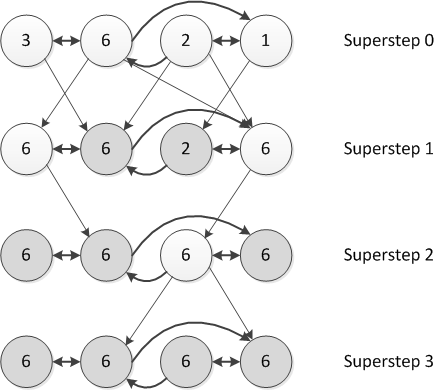
\includegraphics[width=0.5\textwidth]{./img/superstep}
  \caption{Maximum Value Example. Lighter lines are messages. Shaded vertices have voted to halt \cite{pregel}.}
  \label{fig:superstep}
\end{figure}

Figure \ref{fig:superstep} shows an example program in Pregel, which finds the maximum vertex value. Initially, all vertices are active, and send a message to each vertex they are connected directly containing their value. In the next superstep, if a vertex receives a message with a higher value than its currently stored value, then it stores the new higher value, otherwise the vertex deactivates as it currently has a local maximum whilst the program has not terminated. The vertices which did change send their value send a message containing their updated value to their neighbours. In superstep 2, the third vertex activates and changes its value from 2 to 6 as it receives a message containing the value 6. The two active vertices deactivate because they did not receive a message. The third vertex then sends a message to the second and fourth vertices containing the value 6, and in the third superstep, no vertex receiving a message changes its value, so does not need to send a message resulting in all vertices becoming inactive and terminating the program. The maximum value of all the vertices within the graph is now stored in all vertices.

As a Pregel program begins execution, multiple copies of the program start executing on a cluster of machines. A single copy is assigned as the \emph{master} which does not perform any work for the actual program, and instead manages the remaining \emph{worker} copies of the program. The \emph{master} partitions the input graph across the \emph{workers} and instructs the \emph{workers} to perform a superstep. This causes one iteration of the program to occur, and is repeated until all vertices vote-to-halt. The \emph{master} can the instruct each \emph{worker} to save its partition of the graph to memory.

The use of an underlying Bulk Synchonous Parallel model provides the Pregel framework with a simple way to model iteration of graph algorithms, and also provides a simple way to achieve a fault tolerant system. Each superstep in the execution of a Pregel program provides a natural barrier to synchronise each vertex's computation. If a \emph{worker} fails to communicate with the \emph{master} within a defined time period, the \emph{master} assumes that the \emph{worker} has failed, and can restart the program from the checkpoint made at the previous superstep completion, re-partitioning the graph if the failed \emph{worker} is still unavailable.

The Pregel framework also provides some extra useful features called combiners and aggregators. A combiner groups together a series of messages from one vertex to another into a single message containing the result of an operation on these messages. This is to reduce the overhead incurred from sending many messages and then performing the same operation at the receiving vertex. An aggregator is a global data construct, which each vertex has access to its value at each superstep, and the value can be updated at the end of each superstep in time for the next superstep. Aggregators can be used to store information about a graph, such as the number of edges in the graph.

Pregel also supports mutations of the graph an algorithm is being executed on. There are two types of mutations, global and local. A global mutation includes the addition and removal of vertices, as these can affect more that just a single vertex. Global mutations are partially ordered, and the effects of these mutations are seen in the next superstep. A local mutation includes a single vertex adding or removing an edge to another vertex. As these only affect the vertex which is performing these mutations, they happen immediately without any conflicts.

\lstset{language=C++,caption={PageRank algorithm in Pregel \cite{pregel}},label=lst:pregelpagerank,tabsize=2,breaklines=true,breakatwhitespace=true,frame=single}
\begin{lstlisting}[float]
class PageRankVertex
			: public Vertex<double, void, double> {
	public :	
		virtual void Compute(MessageIterator* msgs) {
g			if (superstep() >= 1) {
				double sum = 0;
				for(; !msgs->Done(); msgs->Next())
					sum += msgs->Value();
				*MutableValue() = 0.15 / NumVertices() + 0.85 * sum;
			}
			
			if (superstep() < 30) {
				const int64 n = GetOutEdgeIterator().size();
				SendMessageToAllNeighbors(GetValue() / n);
			} else {
				VoteToHalt();
			}
		}
};					
\end{lstlisting} 

Listing \ref{lst:pregelpagerank} shows how the PageRank algorithm \cite{pagerank} can be written using the Pregel framework. It can clearly be seen how the algorithm works. Each vertex receives a series of messages which contain the PageRank for the vertex which sent the message. The sum of these PageRanks is then computed, and the damping factor applied, and the result is stored as the value of the vertex. This values is then divided by the number of outgoing edges from the vertex, and is then sent as a message to each of the vertices the vertex is connected to.

\subsubsection{Giraph}
\label{sec:res_giraph}
Giraph is a graph processing framework, inspired by Pregel, initially developed at Yahoo!. It has since become an Apache Incubator project\footnote{\url{http://incubator.apache.org/giraph/}}. Giraph is still under development, with more features being added and improved. There are a number of existing solutions to achieve large-scale graph processing, however these also have their own problems.

Graph algorithms can be executed as a sequence of map-reduce jobs in Hadoop, but this suffers from the overheads of repeatedly launching these jobs and the map-reduce model is not a good fit for graph algorithms. Pregel itself has problems in that it requires a separate computing infrastructure, and is also unavailable to non-Google employees. The Message Passage Interface can also be used for graph processing, however it lacks any form of fault tolerance and is consider too generic \cite{giraphtalk}.

\lstset{language=Java,caption={PageRank algorithm in Giraph \cite{giraphtalk}},label=lst:giraphpagerank,tabsize=2,breaklines=true,breakatwhitespace=true,frame=single}
\begin{lstlisting}[float]
public class SimplePageRankVertex extends HadoopVertex<LongWritable, DoubleWritable, FloatWritable, DoubleWritable> {

	public void compute(Iterator<DoubleWritable> msgIterator) {
		double sum = 0;
		
		while (msgIterator.hasNext()) {
			sum += msgIterator.next().get();
		}
		
		setVertexValue(new DoubleWritable((0.15f/getNumVertices()) + 0.85f * sum);
		
		if (getSuperstep() < 30) {
			long edges = getOutEdgeIterator().size();
			
			sendMsgToAllEdges(new DoubleWritable(getVertexValue().get() / edges));
		} else {
			voteToHalt();
		}
	}
}					
\end{lstlisting}

Listing \ref{lst:giraphpagerank} shows the PageRank algorithm \cite{pagerank} produced using Giraph. Strong comparisons can be seen between this, and the Pregel implementation in Listing \ref{lst:pregelpagerank}. Both Listings show that a vertex receives a series of messages, of which the values of each are summer together. A damping factor is then applied and the result stored as the value of the vertex, before this value divided by the number of outgoing edges is sent to each vertex this vertex is connected to.

Small differences can be seen, due to Giraph using Hadoop as an underlying component, such as the type system used in Giraph being composed from Java objects as opposed to primitive date types in Pregel.

There are advantages to Giraph being built on top of Hadoop. Hadoop is being used by a large number of organisations for educational and production uses\footnote{\url{http://wiki.apache.org/hadoop/PoweredBy}} with other organisations providing Hadoop services for users\footnote{\url{http://wiki.apache.org/hadoop/Distributions and Commercial Support}}. This means that Giraph can be deployed onto these clusters with minimal effort required. It also means that Giraph only suffers from Hadoop-based problems, such as the Hadoop namenode and jobtracker being single points of failure for a Hadoop cluster.

Being inspired by Pregel, Giraph also makes use of the Bulk Synchronous Parallel computation model \cite{bsp}. Again for similar reasons to Pregel, the Bulk Synchronous Parallel model provides natural barriers for checkpoints during the execution of programs, and programs can restart from a previous superstep in the case of any failure. Giraph also operates with one copy of the program being designated the \emph{master} and the remaining copies being designated as \emph{workers}. The \emph{master} co-ordinates the \emph{workers}, and also handles the distribution of the input data across the cluster. The \emph{workers} execute the \verb/compute()/ method for every vertex on the partition of data they receive.

Giraph operates as a Map-only job on Hadoop, with there being no Reduce stage. A Giraph job has its own InputFormat and OutputFormat classes which call the user defined Vertex versions of these classes to load the data into each of the \emph{worker} processes.

The basic construct of a Giraph program is similar in style to a Hadoop program. Table \ref{tab:hadoopgiraph} shows this similarity. The \verb/compute()/ method of Giraph is analogous to the \verb/map()/ method of Hadoop. The I, V, E and M represent datatypes to be chosen by the user for their own implementation of Vertex, where:

\begin{itemize}
	\item I $\rightarrow$ VertexId
	\item V $\rightarrow$ VertexValue
	\item E $\rightarrow$ EdgeValue
	\item M $\rightarrow$ MsgValue
\end{itemize}

\begin{table}%
\centering
\begin{tabular}{|m{7.25cm}|m{7.25cm}|} \hline
Hadoop & Giraph \\ \hline
\begin{verbatim}

public class Mapper<
    KEYIN,
    VALUEIN,
    KEYOUT,
    VALUEOUT> {
  void map(KEYIN key,
           VALUEIN value,
           Context context)
           throws IOException,
           InterruptedException;
}
\end{verbatim} &
\begin{verbatim}
public class Vertex<
    I extends WritableComparable,
    V extends Writable,
    E extends Writable,
    M extends Writable> {
  void compute(
    Iterator<M> msgIterator);
}
\end{verbatim} \\
\hline
\end{tabular}
\caption{Comparison between basic Hadoop and Giraph program construct \cite{giraphtalk}}
\label{tab:hadoopgiraph}
\end{table}


\chapter{Specification}

\section{Blah}
% \subsection{MapReduce}
MapReduce is a programming framework designed to simply processing data on large clusters \cite{mapreduce}. MapReduce works by the user supplying two functions, Map and Reduce, which operate in parallel on the data set provided. The Map function processes data from key/value pairs into an intermediate set of key/value pairs, before the Reduce function processes this intermediate set into final key/value pairs.

\lstset{language=C++,caption={Calculating the frequency of words in files using MapReduce \cite{mapreduce}},label=lst:mapreduceexample,tabsize=2,breaklines=true,breakatwhitespace=true,frame=single}
\begin{lstlisting}[float]
map(String key, String value):
	// key: document name
	// value: document contents
	for each word w in value:
		EmitIntermediate(w, ``1'');
		
reduce(String key, Iterator values):
	// key: a word
	// values: a list of counts
	int result = 0;
	for each v in values:
		result += ParseInt(v);
	Emit(AsString(result));	
\end{lstlisting}

Listing \ref{lst:mapreduceexample} is an example MapReduce program which counts the frequency of words within a selection of documents stored on a system. The Map function reads each word, \emph{w}, and emits the word as key/value pair \verb/(w, ``1'')/ to signify that there is an occurrence of \emph{w} at that position. The Reduce function sums together the value each of these emitted key/value pairs, where the key is the same, and emits the sum for each word.

Whilst the example given in Listing \ref{lst:mapreduceexample} uses Strings for the input and output for both of the Map and Reduce functions, it is not necessarily the case that all Map and Reduce functions operate in this way. \cite{mapreduce} explains that the types used by both are linked, as shown by:

\begin{verbatim}
map     (k1, v1)        -> list(k2, v2)
reduce  (k2, list(v2))  -> list(v2)
\end{verbatim}

This states the input keys and values are from a different domain to the output keys and values, which also means that the types used can differ.

MapReduce operates in two phases: The Map phase and the Reduce phase. Initially, the input data is split into small chunks to be assigned to the map tasks. A single map task is designated the master, with the remaining tasks designated as workers. The master assigns each map task a chunk of the input data to process, and once this has been processed, it is assigned more until all the input data has been processed. Once data from a map task has been processed, available reduce tasks then process this into the output data from the MapReduce program.

The MapReduce framework is highly fault tolerant, and is able to cope with multiple worker failure and failure of the master program as well. Each worker is required to periodically communicate with the master, and if no communication is received, then the worker is marked as failed, and its work is redistributed back out to be processed again. In case of the master failing, checkpoints are made and the MapReduce program can restart from the last checkpoint recorded.

\subsubsection{Google File System}
The Google File System, GFS, provides the distributed file system which MapReduce operates with \cite{mapreduce}, but was developed outside of MapReduce to address issues found with previous distributed file systems \cite{gfs}.

The GFS was designed to meet three major points identified with existing distributed file systems \cite{gfs}:
\begin{enumerate}
	\item Component failures are the norm, rather than the exception
	\item Files are huge by traditional standards
	\item Files are mutated by appending new data
\end{enumerate}

As hardware failures are common, the design of the GFS incorporates this, and the system is monitoring itself continually to detect, tolerate, and recover promptly from component failures on a routine basis \cite{gfs}. In addition to this, the system used by Google makes use of inexpensive hardware due to the frequent failures experienced, and as such is a more cost-effective solution than using more expensive tailored hardware.

A GFS cluster is split into a single $master$ and multiple $chunkservers$ and is accessed by multiple $clients$ \cite{gfs}. Files stored in the GFS are split into chunks, which are stored across the cluster on the hard disks located on each chunkserver. By default, each chunk is replicated in the file system three times for reliability of access to data within file system.

Files are stored into the GFS in chunks of size 64MB. This size was chosen to reduce the need to interact with master to find the location of chunks to read data from, and write data to. The larger chunk size also reduces the quantity of metadata stored on the master, which increases the performance of the master as the metadata can be stored in memory, reducing lookup times \cite{gfs}.

The master node maintains the metadata for the file system. This includes the locations of chunks across the file system, and which chunks compose the files stored. The master node communicates with each chunkserver frequently, and if it does not receive a response, the chunkserver is deemed to have failed and any chunks which are then under replicated in the file system are re-replicated to ensure that the minimum number of replications for each chunk are observed.

\subsection{Hadoop}
Hadoop\footnote{\url{http://hadoop.apache.org/}} is framework for performing
distributed computing. It is a free implementation of the MapReduce framework
developed at Google, and is also a top-level project hosted by Apache.

Hadoop has diversified itself from its conception, and is now composed of three
subprojects, Hadoop Common, Haddop Distributed File System, and Hadoop
MapReduce. Hadoop Common providse common utilities which support the other
Hadoop subprojects. The Hadoop Distributed File System is described in more
detail in Section \ref{sec:hdfs}

Hadoop MapReduce is the subproject by which Hadoop itself more known for. It
provides functionality similar to the MapReduce framework developed by Google,
where there exists a $Map$ and a $Reduce$ function which process data across a
cluster.

\subsubsection{Hadoop Distributed File System}
\label{sec:hdfs}
Hadoop also provides a the Hadoop Distributed File System, HDFS. The HDFS is a free implementation of the Google File System, and is designed to be used with Hadoop itself, though can also be used a distributed file system by itself \cite{hdfs}.

The HDFS operates in a similar approach to the operation of Hadoop and the Google File System. There exists a master node, called the NameNode, and many slave nodes, called DataNodes. The NameNode co-ordinates the access of files stored in the HDFS, and also manages the file system namespace. There is usually a DataNode present on each physical node within the cluster. It is the DataNode which control the storage of files on the storage system present on the node, and also controls the reading and writing of files to the HDFS from a user.

The HDFS ensures data integrity through replication of data across different nodes within the cluster. A replication factor is set for the cluster, generally at least 3, which causes all data within the HDFS to be replicated at least that many times. Data within the HDFS is split into blocks, with a large file being represented by many smaller blocks, and it is these blocks which are replicated across the HDFS.

In case of a problem with the HDFS, such as a partial network failure, or hard disk failure, each DataNode is required to periodically message the NameNode which contains a report on all data blocks stored by that DataNode. If there is a failure of some kind, then the NameNode either receives an incomplete message or no message at all. This informs the NameNode that there is a problem with the HDFS and takes appropriate action, including re-replicating the lost data from other DataNodes to new DataNodes.

The HDFS also provides another service called the SecondaryNameNode. The SecondaryNameNode is not a direct failover service to the NameNode. Instead, the SecondaryNameNode takes periodic checkpoints of the state of the NameNode, so that in case of the NameNode failing, a recent copy of the state of the HDFS can be loaded when the NameNode is restarted, which should result in minimal problems with resuming the HDFS.


\chapter{Design}

\section{System Architecture}
Figure \ref{fig:system} contains the intended architecture of DSNAT, and how various components relate to it.

\begin{figure}[htbp]
  \centering
    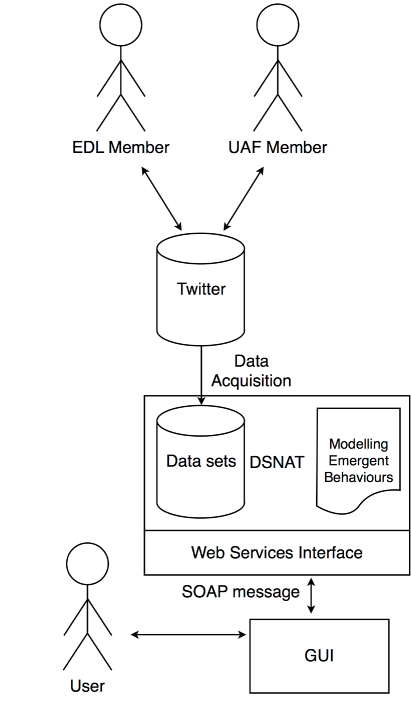
\includegraphics[width=0.4\textwidth]{./img/system}
  \caption{DSNAT system architecture.}
  \label{fig:system}
\end{figure}

The GUI component of the system is being reused from the social network analysis tool \cite{snat} created in the previous year, and what changes will need to me made to adapt it for use with our tool are described in more detail in Section \ref{sec:des_gui}.

We will be collecting data from Twitter from users relating the English Defence League and Unite Against Fascism, amongst other available datasets. The data we acquire will be processed and included into a selection of datasets, from which the tool will then be able to perform various algorithms for analysis.

A portion of this project is research based in the direction of ``Modelling Emergent Behaviours''. With the completion of DSNAT we are hoping to apply the results of this research on much large networks than currently used.

DSNAT forms the core component of the project. Within DSNAT we aiming to have a Hadoop cluster implemented, upon which algorithms for analysing social networks and influence propagation within networks can be executed. The datasets collected during the data acquisition phase of the project will be stored within DSNAT, for processing by users. DSNAT itself will be presented via a web services interface, so that users can remotely connect to DSNAT.
\section{Data Acquisition}

\subsection{Twitter}
Our requirements were as follows:
\begin{itemize}
\item Sufficient data per item to construct a graph
\item Temporal data for use in last year's interface
\item Sufficient nodes to illustrate the cluster’s usefulness
\item Modern, real-world data
\end{itemize}

The social networking site Twitter met all these requirements. As an added bonus, it had information on two groups our customer has an interest in; the English Defence League (EDL) and Unite Against Fascism (UAF). Twitter is easily mapped onto a directed graph as it uses an asymmetric following system where user X can follow user Y without user Y having to follow user X. In addition to collecting the following/followers lists for each user we store the messages they broadcast, their `tweets'. Tweets may be addressed to particular users, and can thus be modelled as edges themselves. In addition to normal, hand-typed tweets there are  `retweets' where the user has essentially endorsed another user’s tweet by repeating it themselves. These can likewise be modelled as directed edges. Along with the text content of a tweet comes a significant amount of metadata such as its timestamp, a unique id, who it\'s addressed to and sometimes geolocational data. Followers have much less information available on them; there is no way to directly tell when a user followed another, or whether a user used to follow another.

\subsubsection{Twitter API}
Twitter provides two main interfaces for developers wishing to harvest data from it; a Representational State Transfer (REST) API and a streaming API. REST is a stateless protocol similar in style to the ubiquitous HTTP/1.1. As a result of prior abuse and overuse The REST API is heavily rate limited. According to the documentation non authenticated calls are limited to 150 requests per hour per IP, and OAuth-authenticated requests are limited to 350 per hour per account. Each of the exposed functions have strict limits on the amount of data they can return; the `statuses/user\_timeline' will only return the 3,200 most recent tweets of a user, and no more than 200 per request. This places a hard limit of 200x350/3200 ~ 20 user's tweets per hour. 

The initial plan was to use the streaming API since it has higher throughput more generous limits and is thus more suited to the quantity of data we wanted to obtain. However, after significant delays and repeated failures to get added to the whitelist we resorted to using the REST API with OAuth for the increased limit.

As a result of the rate limits it will need to be run for time in excess of several days to obtain a substantial amount of data, making it unsuitable for use on our desktop computers. We needed a stand alone script that could be deployed anywhere with minimal setup. SQLite was selected as a lightweight database solution that was easily setup and moved.

\subsubsection{Target Identification Algorithm}
We considered two approaches to identifying members of the target groups; manually identifying a central node and mapping outward from there, or mapping all users who use associated hashtags such as \#UAF. However, preliminary research revealed that many tags have multiple meanings; UAF is commonly used to mean `ugly as f***'. Between tag overloading and news agencies using the \#EDL tag on stories about the english defence league, tags would not have been a substantive foundation for the basic mapping algorithm. Instead, we let the operator specify a central node (easily found via Google's graph-based ranking algorithm) and the algorithm performs a breadth-first-search from there:

\begin{verbatim}
queue.add(startingUser)
while(True)
         target = queue.pop()
         for each user follower/following of target
                 queue.add(user)
         write target\'s tweets/followers/following to db
         write program state to db #added later
\end{verbatim}

Given the low rate at which we could accumulate data, we decided to store all of it to allow for further, unforeseen uses. Simple scripts could then be used to extrapolate graphs in graphml format for our own use, and in MySQL suitable for use in last year\'s visualiser.

\subsection{Stanford Large Network Dataset Collection}
\label{sec:des_snap}
Stanford University host a project called \emph{Stanford Network Analysis Platform}, SNAP.

\begin{quote}
``SNAP is a general purpose network analysis and graph mining library. It is written in C++ and easily scales to massive networks with hundreds of millions of nodes, and billions of edges. It efficiently manipulates large graphs, calculates structural properties, generates regular and random graphs, and supports attributes on nodes and edges.''\footnote{\url{http://snap.stanford.edu}}
\end{quote}

In addition to this library, the SNAP project also hosts a collection of large datasets in the \emph{Stanford Large Network Dataset Collection}\footnote{\url{http://snap.stanford.edu/data}}. This collection of datasets includes a variety of different networks, examples including social networks, communication networks, citation networks, collaboration networks and web graphs.

The majority of these datasets are of the form $NodeId \rightarrow NodeId$, which indicates that these networks cannot be analysed from a temporal perspective. However, the sheer size of some of these networks, notably a LiveJournal network containing 4,847,571 nodes and 68,993,773 edges, and a network of Twitter users from 2009 \cite{kwak10} containing 41.7 million nodes and 1.47 billion edges, should prove DSNAT's viability in performing analysis on large-scale social networks.
\section{Hadoop Cluster}
The largest dataset which was found, on which the tool could potentially perform analysis on, was a snapshot of the entire Twitter network from 2009, which contains 41.7 million nodes and 1.47 billion edges. As a Hadoop cluster can easily be expanded with the addition of extra nodes, the design of the actual cluster itself was fairly simple.

The group met with members of the High Performance \& Scientific Computing about the possibility of a small Hadoop cluster being set up within the department of computer science for us to use, with the hope that the cluster would be large enough to process the highlighted Twitter dataset.

A cluster was implemented for use by the group (see Section \ref{sec:imp_cluster} for further information), which contained a master node, and eight slave nodes. The design of the cluster in this manner, allows the cluster to grow in size if the department desires, but is sufficient for use by the group to analyse graphs of large sizes.
\section{SOAP}

An important part of our project was connecting our code running on the Hadoop cluster to the C\# visualiser created by last year's project group. Therefore, we had to define a means of communicating between these different modules -- as these modules would be running on different machines, this interface had to be exposed as a web service. We chose to implement this communication interface in SOAP; the reason for this choice is detailed below.

\subsection{Choice of SOAP over REST}

[http://www.infoq.com/articles/rest-soap-when-to-use-each]

The two leading candidates for the communication interface were REST and SOAP. These are usually compared side by side, although strictly speaking SOAP is a communications protocol wheras REST is more of an architectural pattern that sits on top of HTTP.

\subsubsection{Advantages of REST}

REST, short for REpresentational State Transfer, is an architectural pattern for using HTTP as a web service. The motivation behind REST is that HTTP already contains a rich vocabulary for manipulating resources -- GET, POST, PUT and so on -- and thus, the logic goes, avoid reimplementing these commands in a complicated new protocol such as SOAP.

[http://www.ajaxonomy.com/2008/xml/web-services-part-1-soap-vs-rest]

The benefits of REST, as defined by [ajaxonomy] and [infoQ], are:
\begin{itemize}
\item It is language and platform agnostic.
\item It is simpler than SOAP, as it does not require an additional messaging
layer.
\item It is closer to the philosopy of the web as originally defined by it's
creator, Tim Berners-Lee.
\item It is able to make use of the built-in capabilities provided by the HTTP
protocol.
\end{itemize}

\subsubsection{Advantages of SOAP}

SOAP, short for Simple Object Access Protocol, is a protocol designed for exchanging structured data via XML. Normally the SOAP framework will abstract away the XML from the end user, using a remote procedure call (RPC) -based interface. An RPC interface is exposed to the application programmer in a simple way; they define a function or method on the server side, and then call that function on the client side. Creating and parsing XML messages is handled by the SOAP library used.

Unlike REST, SOAP can run on top of any transport layer -- this may be HTTP or something else.

The benefits of SOAP [same sources as above], are:
\begin{itemize}
\item Unlike REST, it enables the developer to define their own vocabulary of
verbs to suit the target domain.
\item It is language, platform *and* transport agnostic.
\item It is designed to handle distributed computing environments.
\item It is the predominant standard for web services, meaning there is a
greater level of support in different programming languages.
\item It features built-in error handling.
\end{itemize}

For these reasons, we chose to use SOAP as the communications protocol.

\subsection{Architecture Overview}

[Insert Diagram Here]

The SOAP communication module followed a standard client-server model. The SOAP server (written in Python) would run on the same machine as the Hadoop head node. Python's subprocess module, which lets shell commands be executed from within Python scripts, would be used to allow the SOAP server to control the Hadoop cluster.

Two SOAP clients were written. One was a command line client, also written in Python. The second was the C\#-based visualiser written by last year's project group, which would be modified to send SOAP commands.

During the implementation of the server, one major change to the design proved neccesary; this was modifying it so that it worked in a multi-threaded manner, with one Hadoop task being ran per thread. The reason for this change is detailed in the implementation section below.

Other changes that were made during the design phase included sending large files as base 64-encoding strings, rather than byte arrays, and giving the server the ability to execute algorithms as Python scripts as well as JAR files.

\subsection{Message Structure}

We decided that the API needed to support the following commands:

\begin{itemize}
    \item {\tt upload\_data\_set}

    \begin{description}        
        \item[Arguments] data\_set\_name (string), data\_set (string)
        
        \item[Returns] String
        
        \item[Description] Takes an data\_set (as a base 64-encoded string), and
writes it to a file in the snat\_data\_sets directory on HDFS. Returns
success/failure message.
    \end{description}
    
    \item {\tt upload\_algorithm}

    \begin{description}        
        \item[Arguments] algorithm\_name (string), class\_name (string),
jar\_file (string)
        
        \item[Returns] String
        
        \item[Description] Takes an jar file (as a base 64-encoded string), and
writes it to a file in the algorithms directory (on the regular file system). It
also writes to a text file that keeps of a record of all the uploaded
algorithms. Returns success/failure message. (Note: although the SOAP server can
execute algorithms as either JAR files or Python scripts, currently only JAR
files can be uploaded).
    \end{description}
    
    \item {\tt get\_algorithms}

    \begin{description}        
        \item[Arguments] None
        
        \item[Returns] List[String]
        
        \item[Description] Returns a list of all the algorithms contained in the
algorithms directory.
    \end{description}
    
    \item {\tt get\_data\_sets}

    \begin{description}        
        \item[Arguments] None
        
        \item[Returns] List[String]
        
        \item[Description] Returns a list of all the data sets contained in the
snat\_datasets directory.
    \end{description}
    
    \item {\tt execute\_algorithm}

    \begin{description}        
        \item[Arguments] algorithm\_name (string), data\_set\_name (string),
num\_nodes (integer), command\_line\_args
        
        \item[Returns] Integer
        
        \item[Description] Looks up the algorithm named algorithm\_name. If it
references a JAR file, run a Hadoop job with that JAR. If it references a Python
script, run that script. All jobs are executed in background threads; returns an
integer identifying the thread.
    \end{description}
    
    \item {\tt get\_results}

    \begin{description}        
        \item[Arguments] thread\_id (integer)
        
        \item[Returns] String
        
        \item[Description] Takes a thread\_id referencing a Hadoop job running
in the background. If the job has terminated, returns the output as a base
64-encoded string.
    \end{description}
    
    \item {\tt show\_statys}

    \begin{description}        
        \item[Arguments] required\_data (string)
        
        \item[Returns] String
        
        \item[Description] Currently, takes a port number for one of the Hadoop
logging pages running on localhost, and returns the contents of that page.
    \end{description}
\end{itemize}



\section{Graphical User Interface}
\label{sec:des_gui}

In the approach to creating a suitable interface for the graphs produced by the Hadoop cluster and due the nature of the projects design considerations, which in short is essentially a distributed system with an interface connected via simple object access protocol (SOAP) messages, a few extra design considerations were therefore given to the interface. As the GUI was a continuation of a previous years work, it was first necessary to analyse the structure of the interface, before any modification to the existing code. Another consideration of high importance was the suitability of the graphical visualizer for the graphs and how well the chosen libraries would cope with the size of graphs produced from the datasets we wished to use. A further problem which was analysed in the previous years work review earlier, exposed a complex dependency structure in which the the visualizer operates. This dependency structure lead to the creation of two possible design scenarios in the implementation of the GUI. One design scenario incorporates features of both the original SNAT project possibilities, along with the functionality of this project. 

\subsection{Challenges with continuation of previous project work}
A significant point to mention here is that, while most of the system created for this project is of an original nature, this interface to be used is a continuation of a previous project. This has therefore lead to some issues in modifying the code. Firstly, it was necessary to adjust ones working style to analyse and reverse-engineer the code already created, so that a fuller understand of the structure of the software could be obtained. Secondly, careful analysis of the previous years work had to be undertaken as essentially, our interface is to be developed from the existing tool, regardless of design approach taken. 

\subsection{Graphical User Interface Design Objectives}
As the interface is only one part of a much larger system, it was first necessary to generate some design objectives. This stage is an important consideration when modifying an existing piece of software. Removal or addition of modules or a conflicting of modules could result in the interface becoming non-functional for simply trivial reasons. These "simple" errors can result in massive delays to the implementation process as re-checking of functional base code is necessary to determine whether or not an error is due to a design fault or issue with the previous groups work. Therefore to ensure that the interface was constructed with a reasonable focus in mind on the main objectives of the project, the following design objectives were given to the interface. These objectives were designed to allow the interface: 

\begin{itemize}
	\item To allow suitable connection to the hadoop cluster through use of SOAP messages
	
	\item To connect to the hadoop cluster and perform operations on the cluster such as:
	\begin{itemize}
		\item Upload Algorithms
		\item Upload Dataset
		\item Get Algorithms
		\item Get Dataset
		\item Execute Algorithm
		\item Get Results
		\item Show Statistics
	\end{itemize}
	
	\item To maintain the look and feel of the original interface
	
	\item To follow either one of the two design considerations
\end{itemize}

Therefore the extra objectives for the design of the interface were to:
\begin{itemize}
	\item Remove and insert web-service code into the existing software, while removing any excess code which could cause performance issues
	
	\item Analyse and scale the performance of test data on the visualiser
	
	\item Ensure that the database scheme is reverse-engineered correctly via testing through the visualiser.
	
	\item Ensure that the GUI is suitable to the overall outcome of the project
\end{itemize}

\subsection{The Existing Design}
We shall view the existing SNAT project with regards to only the current projects requirements in terms of the visualisation and GUI. The interface was developed using Microsoft Visual Studio 2010 with the C\# .net framework for the reason that the interface would become simpler to design and construct as the IDE has code completion and management functions. While this module management system is fantastic for developing, in terms of dissecting the code and locating key variables and other important constructs, it was in fact a very troublesome feature. Another issue, was with the compatibility of the IDE with SOAP library's built for C\#, and the lack of them too, however, we shall examine that later.


The first step is to analyse the dependency structure of the GUI in the SNAT project. 

The dependency structure of the GUI starting with the GUI is as show in Table \ref{tab:guidep}.

\begin{table}%
\centering
\begin{tabular}{|l|l|}
\hline
Module & Dependency \\
\hline
GUI	& Network Model, Algorithms API \\
Algorithms API	& Network Model, Database Proxy \\
Network Model	& Database Proxy \\
Database Proxy	& Database \\
Database	& ***No dependencies*** \\
\hline
\end{tabular}
\caption{Dependency of GUI on other SNAT project components}
\label{tab:guidep}
\end{table}

The GUI is heavily dependant on nearly every other module from the previous SNAT project. Each main module is also made up of much smaller submodules which means that in terms of converting the existing interface into a suitable GUI for the distributed SNAT project, a full examination of the previous tools code was required, a very large task. 

Sticking with just the dependency structure of the SNAT code, it was clear that there are two possible designs that could be utilized. The reason for this is because the dependency of certain modules can be offloaded onto the cluster, however, this route should be avoided given the delayed start, as the complexity is dramatically greater than that of the simple implementation which is specified below.

\subsection{GUI Design}

\subsubsection{Design 1}
Dual-function: Combination of SNAT and DSNAT software linked via SOAP messages

The principle behind this design frame of the distributed social network analysis tool's interface is the simplicity in which the goal could be achieved via the use of SOAP messages inserted in key locations, whereby, a web-service would perform the function that the local version would do within the currently available SNA tool. Essentially the process would involve the following as illustrated in Figure \ref{fig:des1}

\begin{figure}%
\centering
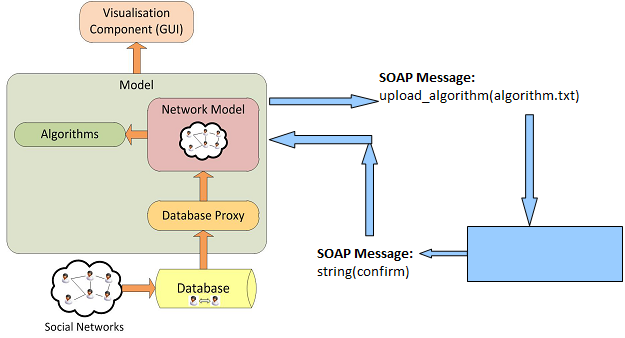
\includegraphics[width=0.6\columnwidth]{./img/des1}%
\caption{Insertion of SOAP messages into current system}%
\label{fig:des1}%
\end{figure}

Code would need to be strategically removed from the existing code to ensure that the visualiser and GUI only view one set of data and system variables at any one time. The overall design we shall not go into much detail, as it is quite simple. The overall code structure of the system would remain the same, however, methods that would have been called on the local software, would instead call a web-service, which should send a SOAP message, detailing the action of the cluster. The data would be processed through the cluster, with results being uploaded to the database, whereby the visualiser should play through the tape produced with statistics either being derived from the data locally, or remotely via another SOAP message communication with the cluster.

Advantages of this design:
\begin{itemize}
	\item Allows for minimal changes to existing code which should provide an easier platform in which debugging can take place
	
	\item Simple addition of a switch could alter connection state with server, e.g. implementation of an offline mode where a local SQL database could be connected
	
	\item Minimal reliance on cluster to process visualisation
	
	\item Safer option than design \#2 with respect to time constant
\end{itemize}

Disadvantages of this desgin:
\begin{itemize}
	\item Visualisation heavily dependent on specification of local system
	
	\item Database handling conducted by local machine
	
	\item Current software may not be compatible in terms of design to incorporate SOAP functionality, however, this is due to the dependencies associated with the rest of the system. Careful consideration of each methods responsibilities and actions should prevent this becoming a problem
\end{itemize}

One disadvantage noted above, is that the visualiser is heavily dependent on the specification of the machine on which the software is locally running on. The main concern with this issue is that, with the size of graphs this project is aiming to achieve in terms of long run goals, a situation where the visualisers performance could be subject to question, is extremely likely. However, testing of the interface with increasing magnitudes of datasets should determine whether or not the current interface visualisation techniques are suitable to this project.

\subsubsection{Design 2}
The second design is radically different from the first, however still manages to incorporate the features and feel of the original interface. As opposed to the design details above, the GUI would work in the following manner. 

The network view model and all functionality stripped from the GUI module and dependency cut. The network model and algorithms modules would move onto the cluster where the graph would be generated. However, this design obviously has some flaws, which is mostly due to the complexity. Figure \ref{fig:des2} represents the system dataflow design.

\begin{figure}%
\centering
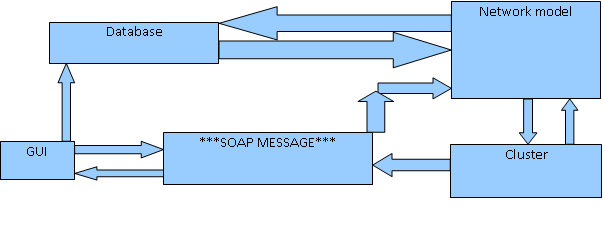
\includegraphics[width=0.6\columnwidth]{./img/des2}%
\caption{Design overview of standalone visualiser client with cluster processed imaging}%
\label{fig:des2}%
\end{figure}

The GUI is the only running module that exists from the SNAT project, with the network view model associated with the cluster rather than the interface. However, this design will not be used for a few simple reasons:

\begin{itemize}
	\item The design is far too complex. This design would require complete re-working of the current network view model and also the cluster design to incorporate the generation of the network view model
	
	\item This design does not alleviate any concerns regarding the current visualiser. As the method of graph visualisation is through the plug-ins GraphSharp and QuickGraph, the visualisation power is only as strong as the system running the plug-ins
	
	\item The cluster will be run on the Linux operating system, which therefore means conversion of or possible running of the code within mono, which is not suitable with some components of the system.
\end{itemize}

An alternative to the current visualiser, is the possible use of cytoscape, an open source network analysis tool. However, this visualisation technique will only be considered depending on the performance testing of the current visualiser.

\subsection{Visual Studio}
The chosen development environment for the DSNAT's GUI was Microsoft Visual Studio 2010 with the C# .net environment. Essentially the same IDE was used and a copy of the project at that point in time, secured from the previous groups website at "http://code.google.com/p/snat/source/browse/trunk/snat/snat/snat.csproj" where the file located at this point would allow an import of the Visual Studio solution.

While the IDE chosen, allowed for quicker analysis of the current project code as it made it easier to follow the reports and guides that were written by the previous group, it had a drawback, as alteration to code generated by other is always a complex and tiresome task, resulting in errors usually caused by misunderstanding of the currently implemented code, further hindered by the complex and the wizard creation style of web-service generation that visual studio provides.

To gain a further understanding of the web-services that can be developed within visual studio, below is an example of a web-service being generated within Microsoft Visual Studio.

\subsub{Web-service generation in Visual Studio}

Pre-requisites:
\begin{itemize}
	\item Internet-information services needs to be running in order for the WSDL to work correctly.
	
	\item Microsoft Visual Studio 2010
\end{itemize}

\subsubsection{Adding a web-service client application in Microsoft Visual Studio 2010}
The first step in creating a web-service in Visual Studio 2010 is to ensure that  the virtual directory and name of the SOAP type is created. As each SOAP type has a web service definition language (WSDL) file associated with it, this is the location in which each method call will be stored and all procedures relating to the functioning of the web-service interface defined. 
Therefore before anything else we must first add a web reference to the project and specify the URL to the virtual name of SOAP type, followed by ``?wsdl''. 

Visual Studio then creates a Web service proxy class and adds it to the project. This proxy class details the methods of the web-service (defined by the WSDL file). By using this proxy class, any of the methods exposed by the virtual name can be invoked. After each request the server sends to the client in the format that was specified for that method during configuration of the virtual name of soap type the data or action requested.

The result of an operation can be returned  as one of the following types: 
\begin{itemize}
	\item XMLElement (System.Xml.XmlElement) or DataSet (System.Data.DataSet) type array 
	
	\item SqlMessage type array elements, which holds error messages that are returned
	
	\item SqlResultCode type array elements, which holds the return value when a UDF that returns a table or a stored procedure is executed 
\end{itemize}

The main data types of the SOAP interface that we shall be using, will be the XMLElement element.

Limitation of using Visual Studio when adding a SOAP reference is that the methods of incorporating the web-service is completely dependent on the style that Microsoft designed for Visual-studio. Another issue is that the insertion of a web-service is extremely complex when compared to that of another library such as Axis Apache 2. 

\section{Emergent Behaviour}

The simulation will be written in Java.
Java was chosen for many reasons, such as:
\begin{itemize}
    \item it is available on all of the most popular computing platforms;
    \item it produces cross-platform applications;
    \item it is easy to package dependencies in one bundle;
    \item there is a wealth of third-party libraries and tools which can be
used.
    \item it has good performance, which is necessary given the scale of the
simulations.
\end{itemize}

The simulation will use the Java Universal Network/Graph Framework
(JUNG),
as the base for the graph implementation.
JUNG is an open-source graph library and contains a lot of data
structures for representing graphs and routines for manipulating the
graphs.
JUNG was chosen for many reasons, including:
\begin{itemize}
    \item it is able to generate many different types of graphs;
    \item it is mature, and has no bugs which would impair the results;
    \item writing bespoke code to handle graphs would be challenging to get
right;
    \item it includes many useful algorithms that can be useful in analysing the
graphs.
\end{itemize}

A `wrapper' class will be written around the JUNG {\tt graph} class in
order to introduce additional functionality that will be required in the
simulation.

Graphs will be generated using JUNG's random graph generators.

Every vertex in the graph will represent an agent in the simulation.
To allow individual vertices to be randomly access in a fast manner,
each vertex will have a unique identifier and be stored in a lookup
data-structure.

Each agent will have a tag and tolerance instance variable to be able to
represent an agent in the graph.
Every agent will also have a {\tt score} instance variable which will be
used to keep track of the success of the agent.
When the agent donates, the cost of donation, $c$, will be subtracted
from the agent's score variable.
When the agent receives a donation, the benefit, $b$, will be added to
the agent's score variable.
This approach allows the success of a given agent to be compared to the
success of another agent by comparing the score variables of each agent.

A class will be created to control the parameters of a simulation---such
as the number of generations to simulate, or the number of interaction
pairings per agent per generation---and to allow multiple simulations to
be run with different parameters in order to compare the results.

The simulation will be started by passing in a set of parameters.
The simulation will then generate a graph and set the initial state of
the simulation according to the parameters passed in.
The simulation will then be run.

\begin{algorithmic}
\While {iterations remain}
    \State Donation()
    \State Reproduction()
\EndWhile
\end{algorithmic}

\includegraphics{./img/mp/AgentVertex.1}


\section{Algorithms}
The algorithms which are implemented for DSNAT will be stored on the cluster for use via the web services interface.

Giraph provides a comprehensive API to implement distributed graph algorithms, because of this we do not see a need to implement a new API to act as a basis for implementing algorithms.

For algorithms which are difficult to express using Giraph and its vertex oriented design, we are able to fall back to using a Hadoop-based approach for implementation.

\subsection{Giraph}

\subsubsection{3-Cliques}
For simplicity reasons, we are only concerning ourselves with identifying 3-cliques within graphs

\subsubsection{Local Clustering Coefficient}

\subsubsection{PageRank}



\subsection{Influence Propagation}

The influence propagation algorithm studied were conceptually simple. However, implementing them in a distributed computing environment like Hadoop proved complex. One major reason for this was that graph algorithms are inherently hard to parallelize. 

Hadoop works best for ``embarrasingly parallel'' problems, that is, tasks which can be broken up into subtasks where there is little dependencies between individual tasks. Graph problems such as influence propogation are inherently about dependencies, as graphs express the relationships between different pieces of data. At some point any graph processing algorithm run in a distributed environment must parition the graph into portions to be run on each indiviual node, and then decide how to communicate between these nodes without causing too slow a bottleneck.

The Pregel framework is one solution to the problem of running graph algorithms on top of Hadoop. As we had used already Pregel for some graph processing problems, we decided to implement the influence propagation algorithms in vanilla Hadoop, to explore the difficulty of implementing graph algorithms without a specialised framework.

\subsubsection{Independent Cascade}

The first step towards implementing the independent cascade algorithm on Hadoop was realising that it was best implemented as multiple tasks, rather than a single task.

Specifically, a simple way of implementing independent cascade is to first ``roll all the dice'' -- that is, decide if influence would successfully pass between each pair of connected nodes -- and then run a standard connected components algorithm.

Therefore, the algorithm was split into two tasks, one to handle the ``dice rolling'', one to handle the connected components. The first task would be run once, whereas the second task would be run iteratively, with the output of one step being fed into the next step. More details can be found below.

\paragraph{Dice Rolling}

The input to this task was a file representing a graph in trivial graph format (TGF). This is a straightforward format that represents one node or edge per line; a representation which allowed the TextInputFormat and TextOutputFormat classes to be utilised for reading and writing the data. These classes allow Hadoop to easily handle text files, where each key-value pair represents one line of text (the key representing the position in the file, and the value representing the actual text).

Example TGF graph:

\begin{verbatim}
1 A false
2 B false
3 C false
4 D true
5 E false
1 2 0.19620324034685735
3 5 0.19051880402243856
3 4 0.12860629863762937
1 2 0.1707108546245374
4 5 0.12539404190086925
2 4 0.18033526297221486
1 5 0.18269135483394416
1 3 0.07440361004495522
2 5 0.13402102761559026
1 4 0.15267731629694137
\end{verbatim}

The first five lines represent the nodes of the graph, in the format: [node id] [node name] [converted at start?]. This graph has 5 nodes, and only node D is set to be converted at the start. The next ten lines represent edges, in the format [node 1] [node 2] [edge weight].

The dice rolling step was then straightforward to implement as a single Hadoop task. All the work was implemented in the map step; the basic algorithm looked like this:

\begin{verbatim}
for each key, value {
  # key is a line number and can be discarded, we only care about the value

  values = parse(value)
  if values represent a node {
    if node is already influenced {
      write(nodeId, 0) # record this node is preinfluenced
    } else {
      # do nothing - we don't need to record this node
    }
  } else if values represent an edge{
    rand = rand(0,1)
    if rand < values.edgeWeight {
      write(node1id, node2id) # this edge is ``live'' and is recorded
      write(node2id, node1id)
    } else {
      # this edge is not live, so we don't need to record it.
    }
  }
}
\end{verbatim}

The reduce step merely implements the identity function and copies over the data from the map step.

The output of this task will then look something like:

\begin{verbatim}
4 0
1 2
2 1
3 4
4 3
4 5
5 4
\end{verbatim}

This might look like a strange way of representing a graph, but it was the most straightforward way to represent a graph using only key/value pairs of integers, and in a way that allows Hadoop to run a connected components algorithm on it.

Lines that end in zero (or a negative number) represent converted nodes. The line ``4 0'' shows that node 4 has been converted. Note that we do not need to record unconverted nodes -- either they are implicitly recorded in the edges or they are completely disconnected from the spanning subgraph created after the dice are rolled, and are irrelevant.

Edges are recorded in the form:

\begin{verbatim}
[node1id] [node2id]
[node2id node1id]
\end{verbatim}

Note that edges are recorded in both directions. The reason for this is explained in the next section.

\paragraph{Connected Components}
[http://blog.piccolboni.info/2011/04/map-reduce-algorithm-for-connected.html]

This step was responsible for taking the spanning subgraph output by the last step and determining which nodes were connected to pre-converted nodes. This is equivalent to the standard connected components problem.

Our implementation for the connected components algorithm was based on a breadth first search. Every node that was connected to a converted node would be marked as converted. This process would then be repeated until all edges had been traversed or were unreachable.

Of course, such an algorithm could not be implemented as a single Hadoop job, and so this task had to be performed iteratively, with the output of one task being fed into the input for the next task. This process would be repeated until the termination condition was met.

This meant that each Hadoop task would represent one iteration of the algorithm; that is, each task would convert all the nodes that were direct neighbours of already converted nodes. The implementation of this was as follows:

The map step merely parsed each line of the file, each containing two integers, and split each line into a key-value pair.

The reduce step performed most of the work. It took advantage of the Hadoop framework, which passes to each reduce task a collection of all the values corresponding to a particular key. Since in our representation keys were nodeIds, that meant that each node would be processed by a different task, and each task would have all the relevant information for it's corresponding node.

This information consisted of:
- whether the node was already converted
- all the edges incident on the node (this was the reason that edges were recorded in both directions).

For example, node number 4 in the above graph corresponded to the following key-value pairs:

\begin{verbatim}
4 0
4 3
4 5
\end{verbatim}

This represents the fact that node 4 had been converted, and that 3 and 5 were neighbouring nodes.

The actual algorithm worked as follows:

\begin{verbatim}
Input(key:integer, values:list(integers)
node1converted? = false
for each value in values {
  node1 = key
  node2 = value

  if node2 <= 0 {
    node1isConverted = true
    convertingNeighbour = node2
  } else {
    neighbours.add(node2)
  }
}

if node1isconverted {
  write(node1, convertingNeighbour) # copy this data from the last iteration
  for neighbour in neighbours {
    write(neighbour, -node1)
    changedNodes++
  } 
} else {
    # node1 is not converted, so nothing changes, so just copy the previous values
    for neighbour in neighbours {
      write(node1, neighbours)
    }            
}
\end{verbatim}

(neighbour, -node1) is recorded for each converted neighbour. The presence of [nodeId] [negativeNumber] indicates that particular node has been converted, and inverting the negative number tells us which node converted it.

changedNodes is a counter, a global variable shared across Hadoop nodes. This counter is used to check for the termination condition; if changedNodes remains zero after an iteration, then execution halts.

A Ruby script was written to run and coordinate the different Hadoop tasks.

\paragraph{Alternatives}

[http://blog.piccolboni.info/2010/07/map-reduce-algorithm-for-connected.html] One alternative way to implement the connected components task was using the PRAM algorithm, as described in [cite]. In theory this allows the connected components of a graph to be found in less iterations.

\subsection{Linear Threshold}

The Linear Threshold implementation follows the same basic pattern as the Independent Cascade implementation, though it only requires one task, which is performed iteratively. Each iteration corresponds to one iteration of the LT algorithm; that is, it counts all the converted neihbours of each unconverted node, and if it is greater than the node's threshold value, the node becomes converted.

Once again, the trickiest part of the algorithm proved to be representing the state of the algorithm in a concise form that could handle both edges and nodes. The data format worked as follows:

Nodes were represented by [nodeId] [threshold]. If the threshold was equal to -1, this represented a node that had already been converted (and so we no longger cared what the threshold value was).

Edges are represented by [node1id] [node2id] [node2converted?]. Once again, edges were recorded in both directions, to ensure that each node would have all the neccesary information at the reduce step.

The algorithm then worked as follows:

The map step simply parsed the input file, setting the key to be the first integer on each line and the value to be the rest. As the value was therefore a Text object, further parsing had to be done in the reduce step. Checking whether this had a noticable effect on performance could be a future avenue for exploration.

The reduce step worked as follows:

\begin{verbatim}
Input: key:integer values:list(text)

node1isOn = false
influence = 0

for value in values {
  data = parse(value)
  if data represents node {
    if data[0] == -1 {
      node1isOn = true
    }
  } else if data represents edge {
    neighbours.add(data[0])
    if data[1] == 1 {
      influence++ \# count converted neighbours
    }
  }
}

if node1isOn \&\& influence >= threshold {
  changedNodes++
  write(key, -1) \# mark this node as converted
  for neighbour in neighbours {
    write(neighbour, ``key 1'') \# mark each neighbours edge so the neighbour's influence will increase on the next reduce step
  }
} else {
  \# nothing happens, so just copy over previous values
}
\end{verbatim}


\chapter{Implementation}

\section{Blah}
% \subsection{MapReduce}
MapReduce is a programming framework designed to simply processing data on large clusters \cite{mapreduce}. MapReduce works by the user supplying two functions, Map and Reduce, which operate in parallel on the data set provided. The Map function processes data from key/value pairs into an intermediate set of key/value pairs, before the Reduce function processes this intermediate set into final key/value pairs.

\lstset{language=C++,caption={Calculating the frequency of words in files using MapReduce \cite{mapreduce}},label=lst:mapreduceexample,tabsize=2,breaklines=true,breakatwhitespace=true,frame=single}
\begin{lstlisting}[float]
map(String key, String value):
	// key: document name
	// value: document contents
	for each word w in value:
		EmitIntermediate(w, ``1'');
		
reduce(String key, Iterator values):
	// key: a word
	// values: a list of counts
	int result = 0;
	for each v in values:
		result += ParseInt(v);
	Emit(AsString(result));	
\end{lstlisting}

Listing \ref{lst:mapreduceexample} is an example MapReduce program which counts the frequency of words within a selection of documents stored on a system. The Map function reads each word, \emph{w}, and emits the word as key/value pair \verb/(w, ``1'')/ to signify that there is an occurrence of \emph{w} at that position. The Reduce function sums together the value each of these emitted key/value pairs, where the key is the same, and emits the sum for each word.

Whilst the example given in Listing \ref{lst:mapreduceexample} uses Strings for the input and output for both of the Map and Reduce functions, it is not necessarily the case that all Map and Reduce functions operate in this way. \cite{mapreduce} explains that the types used by both are linked, as shown by:

\begin{verbatim}
map     (k1, v1)        -> list(k2, v2)
reduce  (k2, list(v2))  -> list(v2)
\end{verbatim}

This states the input keys and values are from a different domain to the output keys and values, which also means that the types used can differ.

MapReduce operates in two phases: The Map phase and the Reduce phase. Initially, the input data is split into small chunks to be assigned to the map tasks. A single map task is designated the master, with the remaining tasks designated as workers. The master assigns each map task a chunk of the input data to process, and once this has been processed, it is assigned more until all the input data has been processed. Once data from a map task has been processed, available reduce tasks then process this into the output data from the MapReduce program.

The MapReduce framework is highly fault tolerant, and is able to cope with multiple worker failure and failure of the master program as well. Each worker is required to periodically communicate with the master, and if no communication is received, then the worker is marked as failed, and its work is redistributed back out to be processed again. In case of the master failing, checkpoints are made and the MapReduce program can restart from the last checkpoint recorded.

\subsubsection{Google File System}
The Google File System, GFS, provides the distributed file system which MapReduce operates with \cite{mapreduce}, but was developed outside of MapReduce to address issues found with previous distributed file systems \cite{gfs}.

The GFS was designed to meet three major points identified with existing distributed file systems \cite{gfs}:
\begin{enumerate}
	\item Component failures are the norm, rather than the exception
	\item Files are huge by traditional standards
	\item Files are mutated by appending new data
\end{enumerate}

As hardware failures are common, the design of the GFS incorporates this, and the system is monitoring itself continually to detect, tolerate, and recover promptly from component failures on a routine basis \cite{gfs}. In addition to this, the system used by Google makes use of inexpensive hardware due to the frequent failures experienced, and as such is a more cost-effective solution than using more expensive tailored hardware.

A GFS cluster is split into a single $master$ and multiple $chunkservers$ and is accessed by multiple $clients$ \cite{gfs}. Files stored in the GFS are split into chunks, which are stored across the cluster on the hard disks located on each chunkserver. By default, each chunk is replicated in the file system three times for reliability of access to data within file system.

Files are stored into the GFS in chunks of size 64MB. This size was chosen to reduce the need to interact with master to find the location of chunks to read data from, and write data to. The larger chunk size also reduces the quantity of metadata stored on the master, which increases the performance of the master as the metadata can be stored in memory, reducing lookup times \cite{gfs}.

The master node maintains the metadata for the file system. This includes the locations of chunks across the file system, and which chunks compose the files stored. The master node communicates with each chunkserver frequently, and if it does not receive a response, the chunkserver is deemed to have failed and any chunks which are then under replicated in the file system are re-replicated to ensure that the minimum number of replications for each chunk are observed.

\subsection{Hadoop}
Hadoop\footnote{\url{http://hadoop.apache.org/}} is framework for performing
distributed computing. It is a free implementation of the MapReduce framework
developed at Google, and is also a top-level project hosted by Apache.

Hadoop has diversified itself from its conception, and is now composed of three
subprojects, Hadoop Common, Haddop Distributed File System, and Hadoop
MapReduce. Hadoop Common providse common utilities which support the other
Hadoop subprojects. The Hadoop Distributed File System is described in more
detail in Section \ref{sec:hdfs}

Hadoop MapReduce is the subproject by which Hadoop itself more known for. It
provides functionality similar to the MapReduce framework developed by Google,
where there exists a $Map$ and a $Reduce$ function which process data across a
cluster.

\subsubsection{Hadoop Distributed File System}
\label{sec:hdfs}
Hadoop also provides a the Hadoop Distributed File System, HDFS. The HDFS is a free implementation of the Google File System, and is designed to be used with Hadoop itself, though can also be used a distributed file system by itself \cite{hdfs}.

The HDFS operates in a similar approach to the operation of Hadoop and the Google File System. There exists a master node, called the NameNode, and many slave nodes, called DataNodes. The NameNode co-ordinates the access of files stored in the HDFS, and also manages the file system namespace. There is usually a DataNode present on each physical node within the cluster. It is the DataNode which control the storage of files on the storage system present on the node, and also controls the reading and writing of files to the HDFS from a user.

The HDFS ensures data integrity through replication of data across different nodes within the cluster. A replication factor is set for the cluster, generally at least 3, which causes all data within the HDFS to be replicated at least that many times. Data within the HDFS is split into blocks, with a large file being represented by many smaller blocks, and it is these blocks which are replicated across the HDFS.

In case of a problem with the HDFS, such as a partial network failure, or hard disk failure, each DataNode is required to periodically message the NameNode which contains a report on all data blocks stored by that DataNode. If there is a failure of some kind, then the NameNode either receives an incomplete message or no message at all. This informs the NameNode that there is a problem with the HDFS and takes appropriate action, including re-replicating the lost data from other DataNodes to new DataNodes.

The HDFS also provides another service called the SecondaryNameNode. The SecondaryNameNode is not a direct failover service to the NameNode. Instead, the SecondaryNameNode takes periodic checkpoints of the state of the NameNode, so that in case of the NameNode failing, a recent copy of the state of the HDFS can be loaded when the NameNode is restarted, which should result in minimal problems with resuming the HDFS.

%\section{Data Acquisition}

%\section{SOAP Messaging}

%\section{Cluster}
%\section{Hadoop Cluster}
\subsection{Requirements}
Hadoop itself does not have any explicit hardware requirements, and is able to run on mainst

Hadoop also very few software requirements and is able to run on both Microsoft Windows and varieties of GNU/Linux. Use of Hadoop on a Windows environment is recommended only as a development platform, as Hadoop has not been well tested as a production platform for Windows. Both development and production have been tested using GNU/Linux environments, and is the recommended for use of Hadoop.

Hadoop only has two explicit software requirements: Java\footnote{\url{http://www.java.com/}} and ssh\footnote{\url{http://www.openssh.com/}}. Hadoop launches each of the services required to manage a cluster as Java processes, and as such requires the Java Runtime Environment 1.6.x to be present. As programs developed using Giraph are written in Java, the Java Development Kit is also required, and includes the Java Runtime Environment. Ssh is required, with sshd running on all nodes, to allow the NameNode to manage all nodes within the cluster. 

Giraph has a few extra requirements of its own. It requires specific versions of Hadoop, Hadoop 0.20.203 or higher, which have security changes applied to them. At the time of the project commencement, Hadoop 0.20.205 had been released\footnote{\date{17th October 2011} - \url{http://hadoop.apache.org/common/releases.html}} as the latest version with the required security changes, and as such has been the version with which development of the project has been made with. During the development of the project, Hadoop reached version 1.0.0\footnote{\date{27th December 2011} - \url{http://hadoop.apache.org/common/releases.html}} but we chose to remain with the existing version of Hadoop so as not to introduce any conflicts with any possible deprecations or changes brought about by the newer version.

Giraph also requires Maven 3\footnote{\url{http://maven.apache.org/}} to be installed to compile the Giraph source code into a usable JAR for submitting jobs with to Hadoop.

\subsection{Single-Node Cluster}
For development purposes single-node cluster \cite{nollsingle}

\begin{figure}[htbp]
  \centering
    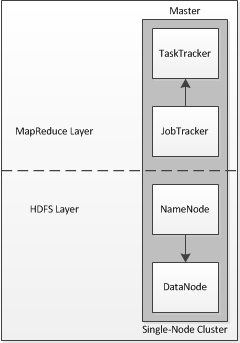
\includegraphics{./img/singlenode}
  \caption{Single-node Hadoop cluster \cite{nollsingle}.}
  \label{fig:singlenode}
\end{figure}

\subsection{Two-Node Cluster}
\cite{nollmulti}

\begin{figure}[htbp]
  \centering
    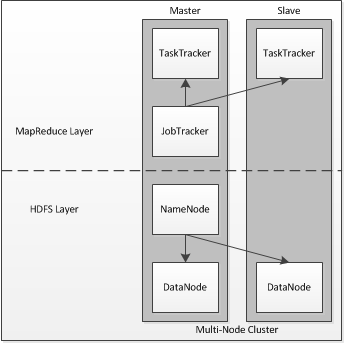
\includegraphics{./img/twonode}
  \caption{Two-nodes Hadoop cluster \cite{nollmulti}.}
  \label{fig:twonode}
\end{figure}

\subsection{Multi-Node Cluster}
At request, a nine machine Hadoop cluster was set up for use during this project in the department of computer science. This cluster composed a master head-node, {\tt hadoopmaster}, and eight slave-nodes, {\tt hadoop\{0-7\}}. 

Being the master, {\tt hadoopmaster} runs the NameNode, JobTracker and SecondaryNameNode processes. Each of the slave-nodes run the DataNode and TaskTracker processes.

HERE WILL BE SOME TECHNICAL SPECS ABOUT THE HADOOP CLUSTER IN THE DEPARTMENT

We did not have direct access to the Hadoop cluster, and were required to {\tt ssh} to a machine located within the department, before {\tt ssh}ing from this machine into the Hadoop cluster. This added an extra level of complexity to access the Hadoop cluster , yet was resolved though use of ssh-keys to allow this \emph{machine-in-the-middle} to send and receive files from hadoopmaster with requiring a password.

\subsubsection{Issues}
One major issue which surfaced when we gained access to the Hadoop cluster in the department of computer science, relating to using Giraph with more than one worker. When a Giraph job is submitted to the cluster using more than one worker, each node which gets used by the job starts a listener which receives messages sent. However, whilst Hadoop jobs submitted to the cluster were able to make use of all nodes within the cluster, Giraph jobs were only able to use one worker, and therefore one node, otherwise an error similar to Listing \ref{lst:girapherror}.

\lstset{language=Java,caption={Giraph error message},label=lst:girapherror,tabsize=2,breaklines=true,breakatwhitespace=true,frame=single}
\begin{lstlisting}[float]
java.net.ConnectException: Call to hadoop6.deepthought.hpsg.dcs.warwick.ac.uk/10.131.56.209:30002 failed on connection exception: java.net.ConnectException: Connection refused
\end{lstlisting}

This error was indicating that there was something wrong with the network configuration, with the most likely problem being that the ports listed in the errors were closed due to a firewall, or similar. However, after some investigation, it turned out that the ports were not blocked and that there was some other issue occuring. Browsing through the user mailing list for Giraph, it became apparent that another user of Giraph was producing the same errors as our cluster\footnote{\url{http://mail-archives.apache.org/mod_mbox/incubator-giraph-user/201112.mbox/\%3C4ED9DDAC.4070208@apache.org\%3E}}. The issue with the use of Giraph on the cluster is how the workers work out which IP address they should listen on, which happens in a different manner to how Hadoop operates, hence why Hadoop jobs would successfully execute whilst Giraph jobs would not. The fix was to remove the mapping from {\tt 127.0.0.1} to {\tt localhost} from the {\tt /etc/hosts} file. With this change made, we were able to successfully able to execute Giraph jobs, making full use of the cluster available.

Another issue which occurred with the cluster is that node {\tt hadoop3} began to produce error messages as show in Listing \ref{lst:hadoop3error}. What was confusing about this error was that all slave nodes, {\tt hadoop\{0-7\}}, are identical in setup and configuration, so for only {\tt hadoop3} to produce serious errors such as this was strange.

\lstset{language=Java,caption={hadoop3 error message},label=lst:hadoop3error,tabsize=2,breaklines=true,breakatwhitespace=true,frame=single}
\begin{lstlisting}[float]
java.lang.Throwable: Child Error
        at org.apache.hadoop.mapred.TaskRunner.run
        (TaskRunner.java:271)
Caused by: java.io.IOException: Task process exit with nonzero status of 134.
        at org.apache.hadoop.mapred.TaskRunner.run
        (TaskRunner.java:258)

attempt_201204171536_0005_m_000005_0: #
attempt_201204171536_0005_m_000005_0: # A fatal error has been detected by the Java Runtime Environment:
attempt_201204171536_0005_m_000005_0: #
attempt_201204171536_0005_m_000005_0: #  SIGSEGV (0xb) at pc=0x00007f4035255dbc, pid=25782, tid=139913655404288
attempt_201204171536_0005_m_000005_0: #
attempt_201204171536_0005_m_000005_0: # JRE version: 7.0_02-b13
attempt_201204171536_0005_m_000005_0: # Java VM: Java HotSpot(TM) 64-Bit Server VM (22.0-b10 mixed mode linux-amd64 compressed oops)
attempt_201204171536_0005_m_000005_0: # Problematic frame:
attempt_201204171536_0005_m_000005_0: # C  [libc.so.6+0x7fdbc]  memcpy+0x4cc
attempt_201204171536_0005_m_000005_0: #
attempt_201204171536_0005_m_000005_0: # Failed to write core dump. Core dumps have been disabled. To enable core dumping, try "ulimit -c unlimited" before starting Java again
attempt_201204171536_0005_m_000005_0: #
attempt_201204171536_0005_m_000005_0: # An error report file with more information is saved as:
attempt_201204171536_0005_m_000005_0: # /home/hduser/hadoop/tmp/mapred/local/taskTracker/hduser/
jobcache/job_201204171536_0005/
attempt_201204171536_0005_m_000005_0/work/
hs_err_pid25782.log
attempt_201204171536_0005_m_000005_0: # [ timer expired, abort... ]
\end{lstlisting}

The approach we took to remedy this was to remove {\tt hadoop3} from operating within the cluster. As {\tt hadoop3} was also a DataNode, the HDFS needed to re-replicate the data held on {\tt hadoop3} across the other seven nodes before they could continue operating as the cluster.

\section{Algorithms}
\subsection{Giraph}
Giraph programs all follow a similar construct. As a minimum, the \verb/compute()/ method needs to be implemented because this is where the algorithms are executed on each vertex within the graph. Listing \ref{lst:giraphstructure} shows the structure of most of the 

\lstset{language=Java,caption={Basic structure of a Giraph program},label=lst:giraphstructure,tabsize=2,breaklines=true,breakatwhitespace=true,frame=single}
\begin{lstlisting}[float]
public class Vertex<I, V, E, M> {
	public void compute(Iterator<M> msgIterator) {}
	
	public static class VertexInputFormat {}
	
	public static class VertexReader {}
	
	public static class VertexOutputFormat {}
	
	public static class VertexWriter {}
	
	public int run(String[] argArray) {}
	
	public static void main (String[] args) {}
}						
\end{lstlisting}

The following briefly describes each of these components

\begin{itemize}

    \item {\tt compute()}

    \begin{description}
        The method which implements the algorithm.
    \end{description}
    
    \item {\tt VertexInputFormat}

    \begin{description}
        Generates splits of the input file to distribute the graph across all workers.
    \end{description}
    
    \item {\tt VertexReader}

    \begin{description}
        Controls reading in the vertices from the input splits.
    \end{description}
    
    \item {\tt VertexOutputFormat}

    \begin{description}
        Controls the output of the graph after computation
    \end{description}
    
    \item {\tt VertexWriter}

    \begin{description}
        Controls the output of the vertices for each worker after computation.
    \end{description}
    
    \item {\tt run()}

    \begin{description}
        Controls the running of the program, including handling of command-line options.
    \end{description}
    
    \item {\tt main()}

    \begin{description}
        The initial method called when the program is submitted as a Hadoop job. Calls the {\tt run()} method.
    \end{description}
    
\end{itemize}

As explained in Section \ref{sec:res_giraph}, a Giraph program is executed as a Hadoop job. This means that in addition to the \verb/compute()/ method being complete, other classes are required to read in and write out the graphs before and after processing to the HDFS.

Following on from the shortest paths example \cite{giraphexample} provided by Apache for Giraph, the decision was taken to use the same JSON\footnote{JavaScript Object Notation \url{http://www.json.org/}} style format to store the graphs as adjacency list structures in the HDFS.

\lstset{language=C,caption={JSON adjacency list representation of a graph},label=lst:json,tabsize=2,breaklines=true,breakatwhitespace=true,frame=single}
\begin{lstlisting}[float]
[1, 0, [[2, 1], [3, 1]]]
[2, 0, [[1, 1], [3, 1]]]
[3, 0, [[1, 1], [2, 1], [4, 1]]]
[4, 0, [[3, 1], [5, 1], [6, 1]]]
[5, 0, [[4, 1], [6, 1]]]
[6, 0, [[4, 1], [5, 1]]]
\end{lstlisting}

Listing \ref{lst:json} represents the graph shown in Figure \ref{fig:json}. The adjacency list representation can be split into three parts, the vertex ID, the vertex value, and a list edges this vertex connects to. As explained in Section \ref{sec:res_giraph}, Giraph only processes directed graphs, hence the need to represent edges in both directions to simulate an undirected graph. The use of this JSON format also maps quite neatly onto the structure of the \verb/Vertex/ class representing a vertex within Giraph, as the vertex ID, vertex value and edges are all easily obtainable.

\begin{figure}[htbp]
  \centering
    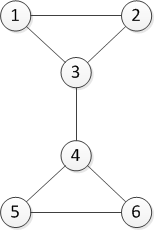
\includegraphics{./img/json}
  \caption{The graph represented by Listing \ref{lst:json}}
  \label{fig:json}
\end{figure}

\lstset{language=Java,caption={Giraph example VertexInputFormat \cite{giraphexample} },label=lst:giraphvertexinput,tabsize=2,breaklines=true,breakatwhitespace=true,frame=single}
\begin{lstlisting}[float]
public static class SimpleShortestPathsVertexInputFormat extends
        TextVertexInputFormat<LongWritable, DoubleWritable, FloatWritable> {
    @Override
    public VertexReader<LongWritable, DoubleWritable, FloatWritable>
            createVertexReader(InputSplit split,
                               TaskAttemptContext context)
                               throws IOException {
        return new SimpleShortestPathsVertexReader(
            textInputFormat.createRecordReader(split, context));
    }
}
\end{lstlisting}

\lstset{language=Java,caption={Giraph example VertexReader \cite{giraphexample} },label=lst:giraphvertexreader,tabsize=2,breaklines=true,breakatwhitespace=true,frame=single,showstringspaces=false}
\begin{lstlisting}[float]
public static class SimpleShortestPathsVertexReader extends
        TextVertexReader<LongWritable, DoubleWritable, FloatWritable> {

    public SimpleShortestPathsVertexReader(
            RecordReader<LongWritable, Text> lineRecordReader) {
        super(lineRecordReader);
    }
    @Override
    public boolean next(MutableVertex<LongWritable,
                        DoubleWritable, FloatWritable, ?> vertex)
            throws IOException, InterruptedException {
        if (!getRecordReader().nextKeyValue()) {
            return false;
        }
        Text line = getRecordReader().getCurrentValue();
        try {
            JSONArray jsonVertex = new JSONArray(line.toString());
            vertex.setVertexId(
                new LongWritable(jsonVertex.getLong(0)));
            vertex.setVertexValue(
                new DoubleWritable(jsonVertex.getDouble(1)));
            JSONArray jsonEdgeArray = jsonVertex.getJSONArray(2);
            for (int i = 0; i < jsonEdgeArray.length(); ++i) {
                JSONArray jsonEdge = jsonEdgeArray.getJSONArray(i);
                Edge<LongWritable, FloatWritable> edge =
                    new Edge<LongWritable, FloatWritable>(
                        new LongWritable(jsonEdge.getLong(0)),
                        new FloatWritable((float) jsonEdge.getDouble(1)));
                vertex.addEdge(edge);
            }
        } catch (JSONException e) {
            throw new IllegalArgumentException(
                ``next: Couldn't get vertex from line `` + line, e);
        }
        return true;
}}
\end{lstlisting}

\lstset{language=Java,caption={Giraph example VertexOutputFormat \cite{giraphexample} },label=lst:giraphvertexoutput,tabsize=2,breaklines=true,breakatwhitespace=true,frame=single,showstringspaces=false}
\begin{lstlisting}[float]
public static class SimpleShortestPathsVertexOutputFormat extends
        TextVertexOutputFormat<LongWritable, DoubleWritable,
        FloatWritable> {

    @Override
    public VertexWriter<LongWritable, DoubleWritable, FloatWritable>
            createVertexWriter(TaskAttemptContext context)
            throws IOException, InterruptedException {
        RecordWriter<Text, Text> recordWriter =
            textOutputFormat.getRecordWriter(context);
        return new SimpleShortestPathsVertexWriter(recordWriter);
    }
}
\end{lstlisting}

\lstset{language=Java,caption={Giraph example VertexWriter \cite{giraphexample} },label=lst:giraphvertexwriter,tabsize=2,breaklines=true,breakatwhitespace=true,frame=single,showstringspaces=false}
\begin{lstlisting}[float]
public static class SimpleShortestPathsVertexWriter extends
        TextVertexWriter<LongWritable, DoubleWritable, FloatWritable> {
    public SimpleShortestPathsVertexWriter(
            RecordWriter<Text, Text> lineRecordWriter) {
        super(lineRecordWriter);
    }

    @Override
    public void writeVertex(BasicVertex<LongWritable, DoubleWritable,
                            FloatWritable, ?> vertex)
            throws IOException, InterruptedException {
        JSONArray jsonVertex = new JSONArray();
        try {
            jsonVertex.put(vertex.getVertexId().get());
            jsonVertex.put(vertex.getVertexValue().get());
            JSONArray jsonEdgeArray = new JSONArray();
            for (Edge<LongWritable, FloatWritable> edge :
                    vertex.getOutEdgeMap().values()) {
                JSONArray jsonEdge = new JSONArray();
                jsonEdge.put(edge.getDestVertexId().get());
                jsonEdge.put(edge.getEdgeValue().get());
                jsonEdgeArray.put(jsonEdge);
            }
            jsonVertex.put(jsonEdgeArray);
        } catch (JSONException e) {
            throw new IllegalArgumentException(
                "writeVertex: Couldn't write vertex " + vertex);
        }
        getRecordWriter().write(new Text(jsonVertex.toString()), null);
    }
}
\end{lstlisting}

%\section{Modelling Emergent Behaviour}


\chapter{Testing}

% \subsection{MapReduce}
MapReduce is a programming framework designed to simply processing data on large clusters \cite{mapreduce}. MapReduce works by the user supplying two functions, Map and Reduce, which operate in parallel on the data set provided. The Map function processes data from key/value pairs into an intermediate set of key/value pairs, before the Reduce function processes this intermediate set into final key/value pairs.

\lstset{language=C++,caption={Calculating the frequency of words in files using MapReduce \cite{mapreduce}},label=lst:mapreduceexample,tabsize=2,breaklines=true,breakatwhitespace=true,frame=single}
\begin{lstlisting}[float]
map(String key, String value):
	// key: document name
	// value: document contents
	for each word w in value:
		EmitIntermediate(w, ``1'');
		
reduce(String key, Iterator values):
	// key: a word
	// values: a list of counts
	int result = 0;
	for each v in values:
		result += ParseInt(v);
	Emit(AsString(result));	
\end{lstlisting}

Listing \ref{lst:mapreduceexample} is an example MapReduce program which counts the frequency of words within a selection of documents stored on a system. The Map function reads each word, \emph{w}, and emits the word as key/value pair \verb/(w, ``1'')/ to signify that there is an occurrence of \emph{w} at that position. The Reduce function sums together the value each of these emitted key/value pairs, where the key is the same, and emits the sum for each word.

Whilst the example given in Listing \ref{lst:mapreduceexample} uses Strings for the input and output for both of the Map and Reduce functions, it is not necessarily the case that all Map and Reduce functions operate in this way. \cite{mapreduce} explains that the types used by both are linked, as shown by:

\begin{verbatim}
map     (k1, v1)        -> list(k2, v2)
reduce  (k2, list(v2))  -> list(v2)
\end{verbatim}

This states the input keys and values are from a different domain to the output keys and values, which also means that the types used can differ.

MapReduce operates in two phases: The Map phase and the Reduce phase. Initially, the input data is split into small chunks to be assigned to the map tasks. A single map task is designated the master, with the remaining tasks designated as workers. The master assigns each map task a chunk of the input data to process, and once this has been processed, it is assigned more until all the input data has been processed. Once data from a map task has been processed, available reduce tasks then process this into the output data from the MapReduce program.

The MapReduce framework is highly fault tolerant, and is able to cope with multiple worker failure and failure of the master program as well. Each worker is required to periodically communicate with the master, and if no communication is received, then the worker is marked as failed, and its work is redistributed back out to be processed again. In case of the master failing, checkpoints are made and the MapReduce program can restart from the last checkpoint recorded.

\subsubsection{Google File System}
The Google File System, GFS, provides the distributed file system which MapReduce operates with \cite{mapreduce}, but was developed outside of MapReduce to address issues found with previous distributed file systems \cite{gfs}.

The GFS was designed to meet three major points identified with existing distributed file systems \cite{gfs}:
\begin{enumerate}
	\item Component failures are the norm, rather than the exception
	\item Files are huge by traditional standards
	\item Files are mutated by appending new data
\end{enumerate}

As hardware failures are common, the design of the GFS incorporates this, and the system is monitoring itself continually to detect, tolerate, and recover promptly from component failures on a routine basis \cite{gfs}. In addition to this, the system used by Google makes use of inexpensive hardware due to the frequent failures experienced, and as such is a more cost-effective solution than using more expensive tailored hardware.

A GFS cluster is split into a single $master$ and multiple $chunkservers$ and is accessed by multiple $clients$ \cite{gfs}. Files stored in the GFS are split into chunks, which are stored across the cluster on the hard disks located on each chunkserver. By default, each chunk is replicated in the file system three times for reliability of access to data within file system.

Files are stored into the GFS in chunks of size 64MB. This size was chosen to reduce the need to interact with master to find the location of chunks to read data from, and write data to. The larger chunk size also reduces the quantity of metadata stored on the master, which increases the performance of the master as the metadata can be stored in memory, reducing lookup times \cite{gfs}.

The master node maintains the metadata for the file system. This includes the locations of chunks across the file system, and which chunks compose the files stored. The master node communicates with each chunkserver frequently, and if it does not receive a response, the chunkserver is deemed to have failed and any chunks which are then under replicated in the file system are re-replicated to ensure that the minimum number of replications for each chunk are observed.

\subsection{Hadoop}
Hadoop\footnote{\url{http://hadoop.apache.org/}} is framework for performing
distributed computing. It is a free implementation of the MapReduce framework
developed at Google, and is also a top-level project hosted by Apache.

Hadoop has diversified itself from its conception, and is now composed of three
subprojects, Hadoop Common, Haddop Distributed File System, and Hadoop
MapReduce. Hadoop Common providse common utilities which support the other
Hadoop subprojects. The Hadoop Distributed File System is described in more
detail in Section \ref{sec:hdfs}

Hadoop MapReduce is the subproject by which Hadoop itself more known for. It
provides functionality similar to the MapReduce framework developed by Google,
where there exists a $Map$ and a $Reduce$ function which process data across a
cluster.

\subsubsection{Hadoop Distributed File System}
\label{sec:hdfs}
Hadoop also provides a the Hadoop Distributed File System, HDFS. The HDFS is a free implementation of the Google File System, and is designed to be used with Hadoop itself, though can also be used a distributed file system by itself \cite{hdfs}.

The HDFS operates in a similar approach to the operation of Hadoop and the Google File System. There exists a master node, called the NameNode, and many slave nodes, called DataNodes. The NameNode co-ordinates the access of files stored in the HDFS, and also manages the file system namespace. There is usually a DataNode present on each physical node within the cluster. It is the DataNode which control the storage of files on the storage system present on the node, and also controls the reading and writing of files to the HDFS from a user.

The HDFS ensures data integrity through replication of data across different nodes within the cluster. A replication factor is set for the cluster, generally at least 3, which causes all data within the HDFS to be replicated at least that many times. Data within the HDFS is split into blocks, with a large file being represented by many smaller blocks, and it is these blocks which are replicated across the HDFS.

In case of a problem with the HDFS, such as a partial network failure, or hard disk failure, each DataNode is required to periodically message the NameNode which contains a report on all data blocks stored by that DataNode. If there is a failure of some kind, then the NameNode either receives an incomplete message or no message at all. This informs the NameNode that there is a problem with the HDFS and takes appropriate action, including re-replicating the lost data from other DataNodes to new DataNodes.

The HDFS also provides another service called the SecondaryNameNode. The SecondaryNameNode is not a direct failover service to the NameNode. Instead, the SecondaryNameNode takes periodic checkpoints of the state of the NameNode, so that in case of the NameNode failing, a recent copy of the state of the HDFS can be loaded when the NameNode is restarted, which should result in minimal problems with resuming the HDFS.

\section{Emergent Behaviours}

In order to validate the results, we compared the results we obtained against the results presented in the papers by Griffiths and Luck. We consistently found that the donation rate followed the same trends as the original papers, however we noticed that in our implementation the donation rate was higher in all the experiments.

In the following experiments, the donation rate was averaged over 10 runs, each with 1000 generations.

The first test we performed was to test the basic RCA algorithm against the modified one presented in Griffiths 2008. We based our experiments off the same experiments presented in the paper, each of which plot donation rate against: context influence (figure ), rewire proportion (figure ), population size (figure ), interaction pairings per generation (figure ) and neighbourhood size (figure ).

The donation rate against context influence shows that the donation rate increases with context influence, and closely mirrors the values for donation rate presented in the original paper. These results can be seen in figure .

In a population of 10\% cheaters, the rewire proportion exhibited a similar effect on the donation rate as was presented in the original paper, as shown in figure . It can be seen in the graph that with the random rewire strategy, the rewire proportion has no effect on the donation rate. The random replace worst, individual replace worst and group replace worst exhibit a similar behaviour, when the rewire proportion is 0, the donation rate is the same as the random rewire strategy but when the rewire proportion is increased, the donation rate jumps higher. As presented in the original paper, when the rewire proportion nears 1, the donation rate begins to drop again.

The graph of population size against donation rate, figure , shows that the population size makes no difference to the overall donation rate.

The number of interaction pairings per generation also has little effect on the donation rate as shown in figure .

From the graph that shows the neighbourhood size against donation rate, figure , it can be seen that the donation rate is fairly similar for small neighbourhoods, but there is a drop in the donation rate when the neighbourhood size reaches 50.

From these results, we can see that the implementation performs similarly to that of the original papers.

\chapter{Results}

\section{Blah}
% \subsection{MapReduce}
MapReduce is a programming framework designed to simply processing data on large clusters \cite{mapreduce}. MapReduce works by the user supplying two functions, Map and Reduce, which operate in parallel on the data set provided. The Map function processes data from key/value pairs into an intermediate set of key/value pairs, before the Reduce function processes this intermediate set into final key/value pairs.

\lstset{language=C++,caption={Calculating the frequency of words in files using MapReduce \cite{mapreduce}},label=lst:mapreduceexample,tabsize=2,breaklines=true,breakatwhitespace=true,frame=single}
\begin{lstlisting}[float]
map(String key, String value):
	// key: document name
	// value: document contents
	for each word w in value:
		EmitIntermediate(w, ``1'');
		
reduce(String key, Iterator values):
	// key: a word
	// values: a list of counts
	int result = 0;
	for each v in values:
		result += ParseInt(v);
	Emit(AsString(result));	
\end{lstlisting}

Listing \ref{lst:mapreduceexample} is an example MapReduce program which counts the frequency of words within a selection of documents stored on a system. The Map function reads each word, \emph{w}, and emits the word as key/value pair \verb/(w, ``1'')/ to signify that there is an occurrence of \emph{w} at that position. The Reduce function sums together the value each of these emitted key/value pairs, where the key is the same, and emits the sum for each word.

Whilst the example given in Listing \ref{lst:mapreduceexample} uses Strings for the input and output for both of the Map and Reduce functions, it is not necessarily the case that all Map and Reduce functions operate in this way. \cite{mapreduce} explains that the types used by both are linked, as shown by:

\begin{verbatim}
map     (k1, v1)        -> list(k2, v2)
reduce  (k2, list(v2))  -> list(v2)
\end{verbatim}

This states the input keys and values are from a different domain to the output keys and values, which also means that the types used can differ.

MapReduce operates in two phases: The Map phase and the Reduce phase. Initially, the input data is split into small chunks to be assigned to the map tasks. A single map task is designated the master, with the remaining tasks designated as workers. The master assigns each map task a chunk of the input data to process, and once this has been processed, it is assigned more until all the input data has been processed. Once data from a map task has been processed, available reduce tasks then process this into the output data from the MapReduce program.

The MapReduce framework is highly fault tolerant, and is able to cope with multiple worker failure and failure of the master program as well. Each worker is required to periodically communicate with the master, and if no communication is received, then the worker is marked as failed, and its work is redistributed back out to be processed again. In case of the master failing, checkpoints are made and the MapReduce program can restart from the last checkpoint recorded.

\subsubsection{Google File System}
The Google File System, GFS, provides the distributed file system which MapReduce operates with \cite{mapreduce}, but was developed outside of MapReduce to address issues found with previous distributed file systems \cite{gfs}.

The GFS was designed to meet three major points identified with existing distributed file systems \cite{gfs}:
\begin{enumerate}
	\item Component failures are the norm, rather than the exception
	\item Files are huge by traditional standards
	\item Files are mutated by appending new data
\end{enumerate}

As hardware failures are common, the design of the GFS incorporates this, and the system is monitoring itself continually to detect, tolerate, and recover promptly from component failures on a routine basis \cite{gfs}. In addition to this, the system used by Google makes use of inexpensive hardware due to the frequent failures experienced, and as such is a more cost-effective solution than using more expensive tailored hardware.

A GFS cluster is split into a single $master$ and multiple $chunkservers$ and is accessed by multiple $clients$ \cite{gfs}. Files stored in the GFS are split into chunks, which are stored across the cluster on the hard disks located on each chunkserver. By default, each chunk is replicated in the file system three times for reliability of access to data within file system.

Files are stored into the GFS in chunks of size 64MB. This size was chosen to reduce the need to interact with master to find the location of chunks to read data from, and write data to. The larger chunk size also reduces the quantity of metadata stored on the master, which increases the performance of the master as the metadata can be stored in memory, reducing lookup times \cite{gfs}.

The master node maintains the metadata for the file system. This includes the locations of chunks across the file system, and which chunks compose the files stored. The master node communicates with each chunkserver frequently, and if it does not receive a response, the chunkserver is deemed to have failed and any chunks which are then under replicated in the file system are re-replicated to ensure that the minimum number of replications for each chunk are observed.

\subsection{Hadoop}
Hadoop\footnote{\url{http://hadoop.apache.org/}} is framework for performing
distributed computing. It is a free implementation of the MapReduce framework
developed at Google, and is also a top-level project hosted by Apache.

Hadoop has diversified itself from its conception, and is now composed of three
subprojects, Hadoop Common, Haddop Distributed File System, and Hadoop
MapReduce. Hadoop Common providse common utilities which support the other
Hadoop subprojects. The Hadoop Distributed File System is described in more
detail in Section \ref{sec:hdfs}

Hadoop MapReduce is the subproject by which Hadoop itself more known for. It
provides functionality similar to the MapReduce framework developed by Google,
where there exists a $Map$ and a $Reduce$ function which process data across a
cluster.

\subsubsection{Hadoop Distributed File System}
\label{sec:hdfs}
Hadoop also provides a the Hadoop Distributed File System, HDFS. The HDFS is a free implementation of the Google File System, and is designed to be used with Hadoop itself, though can also be used a distributed file system by itself \cite{hdfs}.

The HDFS operates in a similar approach to the operation of Hadoop and the Google File System. There exists a master node, called the NameNode, and many slave nodes, called DataNodes. The NameNode co-ordinates the access of files stored in the HDFS, and also manages the file system namespace. There is usually a DataNode present on each physical node within the cluster. It is the DataNode which control the storage of files on the storage system present on the node, and also controls the reading and writing of files to the HDFS from a user.

The HDFS ensures data integrity through replication of data across different nodes within the cluster. A replication factor is set for the cluster, generally at least 3, which causes all data within the HDFS to be replicated at least that many times. Data within the HDFS is split into blocks, with a large file being represented by many smaller blocks, and it is these blocks which are replicated across the HDFS.

In case of a problem with the HDFS, such as a partial network failure, or hard disk failure, each DataNode is required to periodically message the NameNode which contains a report on all data blocks stored by that DataNode. If there is a failure of some kind, then the NameNode either receives an incomplete message or no message at all. This informs the NameNode that there is a problem with the HDFS and takes appropriate action, including re-replicating the lost data from other DataNodes to new DataNodes.

The HDFS also provides another service called the SecondaryNameNode. The SecondaryNameNode is not a direct failover service to the NameNode. Instead, the SecondaryNameNode takes periodic checkpoints of the state of the NameNode, so that in case of the NameNode failing, a recent copy of the state of the HDFS can be loaded when the NameNode is restarted, which should result in minimal problems with resuming the HDFS.

Moofoo

\chapter{Evaluation}

\section{Project Management}
For a project of this size, involving multiple people, a structured approach to organising how development of the project occurred was required

\subsection{Communication}
An important aspect of any project is communication between all parties involved. For this project, this included ourselves, but also our project supervisors.

Once a week we met with our project supervisors to discuss progress made from the previous meeting, and how progress would develop during the next week. These meetings also served as platform to display results of development of some aspects of the project, and directions for research in these areas could be suggested. Minutes from meetings can be found in Appendix \ref{sec:minutes}.

A single group email account was created: \href{mailto:warwicksna@gmail.com}{warwicksna@gmail.com}. This allowed members of the group, and our supervisors, to quickly contact each member of the group as any emails sent to this account were forwarded to all group members.

During the Easter vacation, the group continued the weekly meetings, without direct communication with our supervisors, using Google+ Hangouts. Google+ Hangouts provided an online system where each member of the group could join a chatroom style environment to discuss project development use voice and/or video communications. These meetings within the holiday were followed up with a summary email to the group email account and our project supervisors to ensure that anyone unavailable to make the meeting could be informed of what had been discussed.

\subsection{Group Management}
Each member within the group had a defined role for the development of the project as explained below:

\paragraph{James Michael}


\paragraph{James Kettle}
This member, in addition with Isaac Lewis, was involved with the design and implementation of the SOAP server and client.

This member also implemented scripts which used the Twitter API to collect data on users related to the EDL and UAF, and process the results into the \verb/graphml/ format.

\paragraph{Matthew Cranham}
This member of the group was involved with the design and implementation of the majority of the algorithms running on the cluster. 

This member also became responsible for maintaining the Hadoop cluster to ensure that it performed correctly. One serious issue which occurred with the cluster was that algorithms implemented using the Apache Giraph library would not run, which was fixed through editing a networking configuration file on each machine within the cluster.

Following the implementation of the algorithms and the acquisition of data, it fell to this member to perform analysis on multiple datasets to investigate not only the structure and properties of these datasets, but also the tool developed as an environment to perform analysis of large social networks.

\paragraph{Isaac Lewis}
This member, in addition to James Kettle, was involved in designing and implementing the SOAP server and SOAP client. They also had a role in implementing influence propagation algorithms to execute on the cluster.

\paragraph{Simon Burns}
This member of the group worked on further developing the user interface developed by last year's group. This involved attempting to making the visualisation component of the user interface a stand-alone component so that it could be reused for this project to visualise networks being analysed on the cluster.
%\section{Objectives}
Our project had a series of objectives to meet in order to be a success. This section details these objectives and identifies whether they were met

\subsection{DSNAT}
DSNAT had both system and research oriented objectives. The system objectives are analysed first:

\begin{enumerate}
  \item Provides the ability to analyse social networks of a much larger scale than possible with SNAT
  
  The use of a cluster of computers to perform analysis of network instantly allows computation on a much larger scale to take place. With SNAT having only been recorded as processing data regarding Enron, which consisted of 36,692 nodes and 367,662 edges, DSNAT has been shown to process the Patent Citation network consisting of 3,774,768 nodes and 16,518,948 edges.
  		
  \item Is presented via a web services interface to allow computation to occur remotely
  
  Interaction with DSNAT is possible using the command line SOAP client produced
  
  \item Utilises data collected for the purpose of the project, and provides the ability for users to supply their own data for analysis
  
  This has been achieved through the collection of data regarding the EDL and UAF, which was processed and uploaded into DSNAT for analysis. Due to time and system constraints, the quantity of data collected from Twitter is small in comparison to the size of the networks can be analysed on DSNAT, yet the results produced are worthwhile.
  
  \item Provide a basis for modelling emergent behaviour on a larger scale
  
  This has partly been achieved. DSNAT is able to process graphs and networks of a large scale, yet the modelling of emergent behaviours needs to be adapted to either the MapReduce or Pregel paradigm before it can be used on DSNAT.
\end{enumerate}

These are the research objectives for DSNAT:

\begin{enumerate}
	\item Clustering: $k$-cliques, $k$-trusses, Kernigham-Lin algorithm and Clustering coefficients
	
	This has been partly achieved. DSNAT has algorithms implemented which can identify 3-cliques and compute various clustering coefficients. $k$-trusses and the Kerningham-Lin algorithm were not implemented
	
	\item Centrality: Betweenness centrality and PageRank
	
	The Giraph library came supplied with a simplified version of the PageRank algorithm, which has been improved slightly. The betweenness centrality measure algorithms remains unimplemented
	\item Influence Propagation: Independent Cascade and Linear Threshold
	
	This has been achieved. Both the independent cascade model and the linear threshold model have been implemented for DSNAT, with promising results produced
\end{enumerate}

The reason behind some algorithms not having been implemented is due to the difficulty encountered in implementing algorithms to operate in a parallelised manner. The Giraph framework makes some algorithms nearly trivial to parallelise, but makes others seemingly impossible due to the lack of a central data-structure which can be referred to.

The algorithms which have been implemented, have been used to analyse the various datasets which were collected and the results can be observed of these can be observed in Section \ref{sec:results_datasets}.

\subsection{Emergent Behaviours}

\begin{enumerate}
	\item Research on Modelling Emergent Behaviours;
	
	We performed this research, and focused on simulations of tag-based cooperation.
	
	\item Evaluate research;
	
	We identified that the previous research had only been performed on graphs with random topologies.
	
	\item Design an algorithm to simulate strategies of disruption;
	
	We designed software to perform the simulations presented in the papers we read, and also to look at extending the research that had already been performed.
	
	\item Implement the algorithm on top of the distributed social network analysis tool;
	
	We were able to create a software simulation and use it as a platform to further extend the existing research.
	We did not create this software using the distributed social network analysis tool that was created as part of this project due to the time constraints.
	
	\item Evaluate results.
	
	We were able to evaluate the results of the extensions we made to the research.
\end{enumerate}
%\input{./tex/eval_timeplan}
%\input{./tex/eval_learning}
%\section{Lessons}


\subsection{Hadoop}

\subsection{Emergent Behaviour}

\subsection{SOAP}

\subsection{Influence Propogation}

\subsection{Visualiser}

\subsection{Algorithms}


\section{Future Extensions}


\subsection{Hadoop}

\subsection{Emergent Behaviour}

\subsection{SOAP}

\begin{itemize}
	\item Extending the showStatus method so that it does more than merely echo the logging pages. A more useful method might be able to parse these logging pages, to return a particular piece of information.
	\item Allowing algorithms to be uploaded as Python scripts (that is, Python scripts that can call Hadoop jobs). One reason this was not done was because an implementation would likely be fairly brittle and depend on scripts being written for the particular installation of Hadoop. If a robust solution could be implemented, it would be useful for anyone who wished to develop a multi-stage Hadoop task. 
\end{itemize}

\subsection{Influence Propagation}

\begin{itemize}
	\item One influence propagation model that was not explored was the diminishing cascade model. As this is a realistic model for many situations---i.e. people are often unlikely to be converted to an idea after a previous failed conversion attempt. Implementing this model in Hadoop could be interesting.
	\item Running more experiments on the implemented algorithms. Graphs with different properties would be an interesting avenue to explore, i.e. varying the clustering coefficient, average node degree, or edge weighting. Some papers found there to be a ``tipping point'' in properties such as average edge weights where influence cascades suddenly turned into epidemics; it would be interesting to explore if the same held true for other properties. In [digg paper], it was found that the presence or absence of influence ``epidemics'' depended strongly on the structure of the networks.
	\item Performance testing the implemented algorithms.
\end{itemize}

\subsection{Visualiser}

\subsection{Algorithms}
One area of the project which is a bit lacking, is the number of algorithms implemented to execute on the cluster. 




% Bibliography
\nocite{*} % Includes material read, but no cited
\bibliographystyle{plainnat}

% I recommend we have .bib file for each of us
\bibliography{./bib/matt,./bib/jamesm,./bib/jamesk,./bib/simon}

% Appendix
\appendix
\chapter{Twitter Harvesting User Guide}
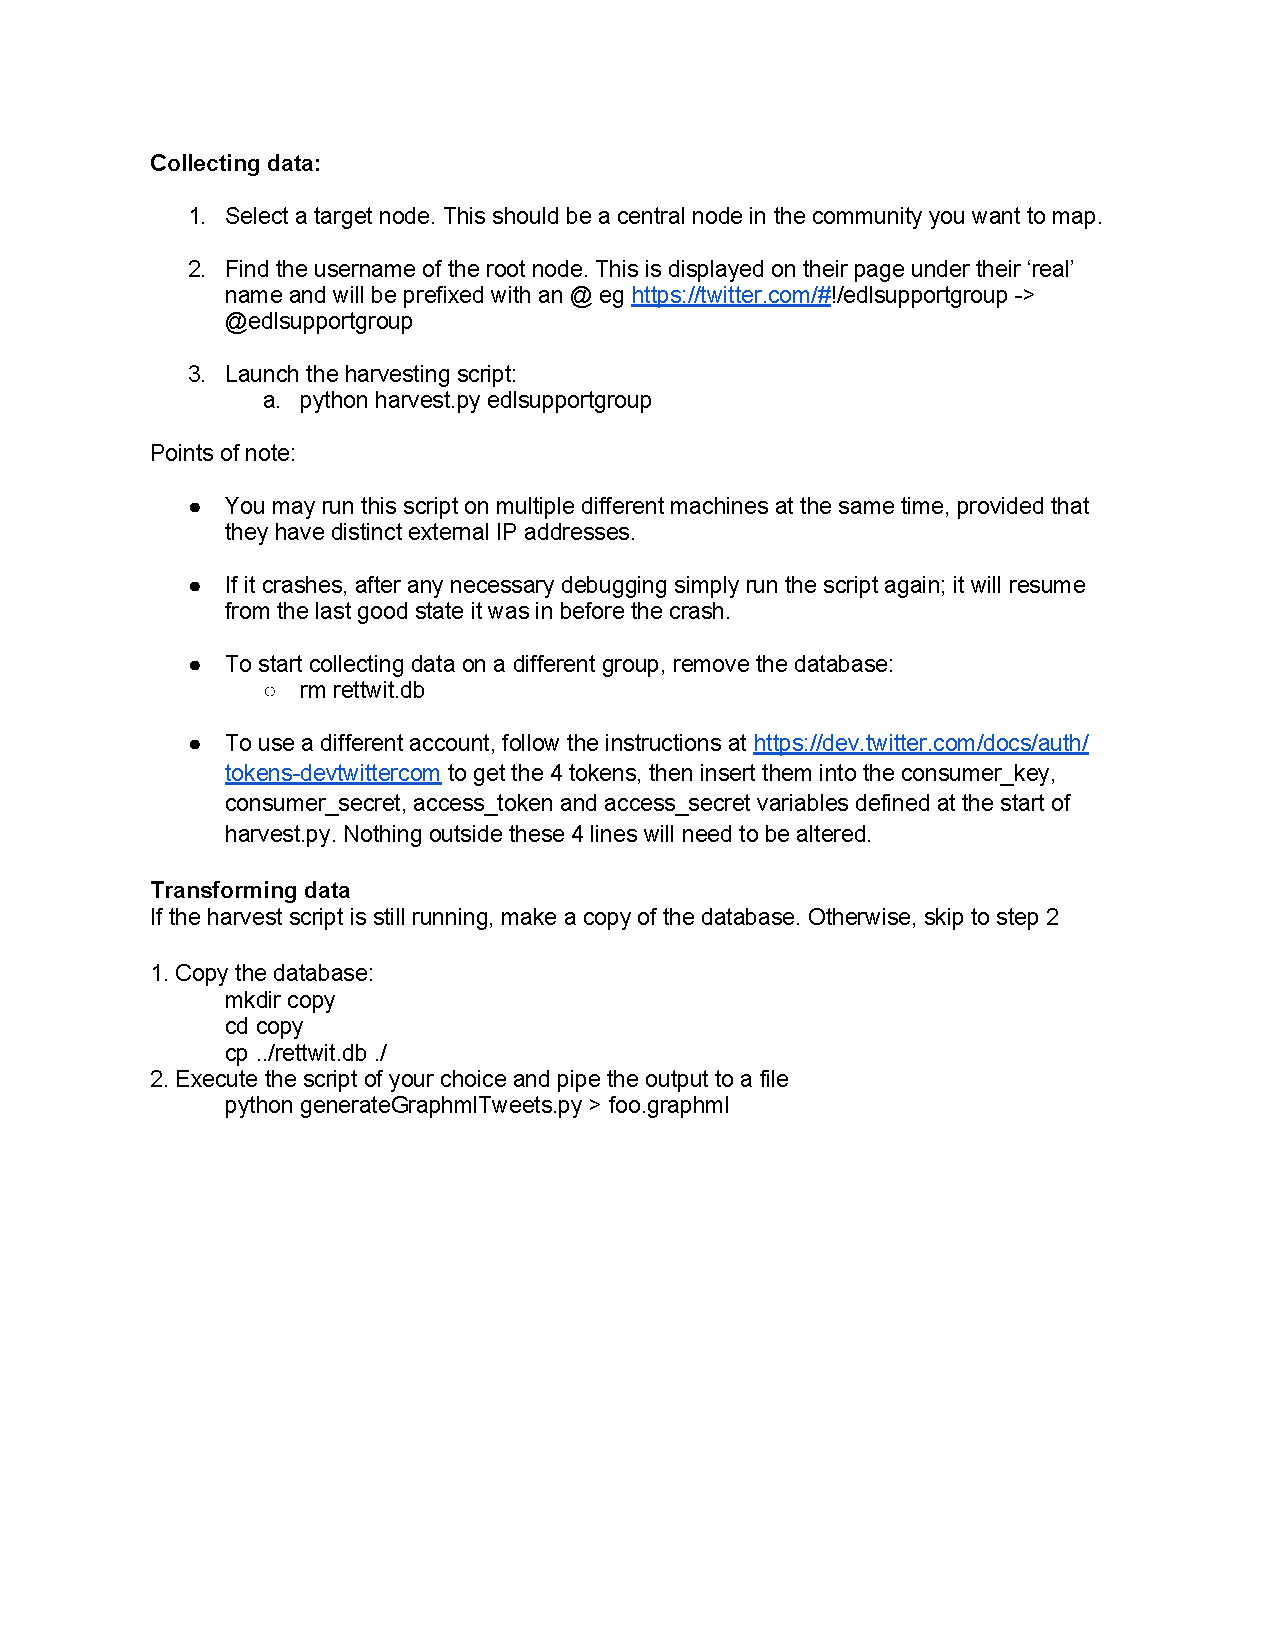
\includepdf[pages=-]{./pdf/harvest}

\chapter{Minutes of Meetings}
\label{sec:minutes}
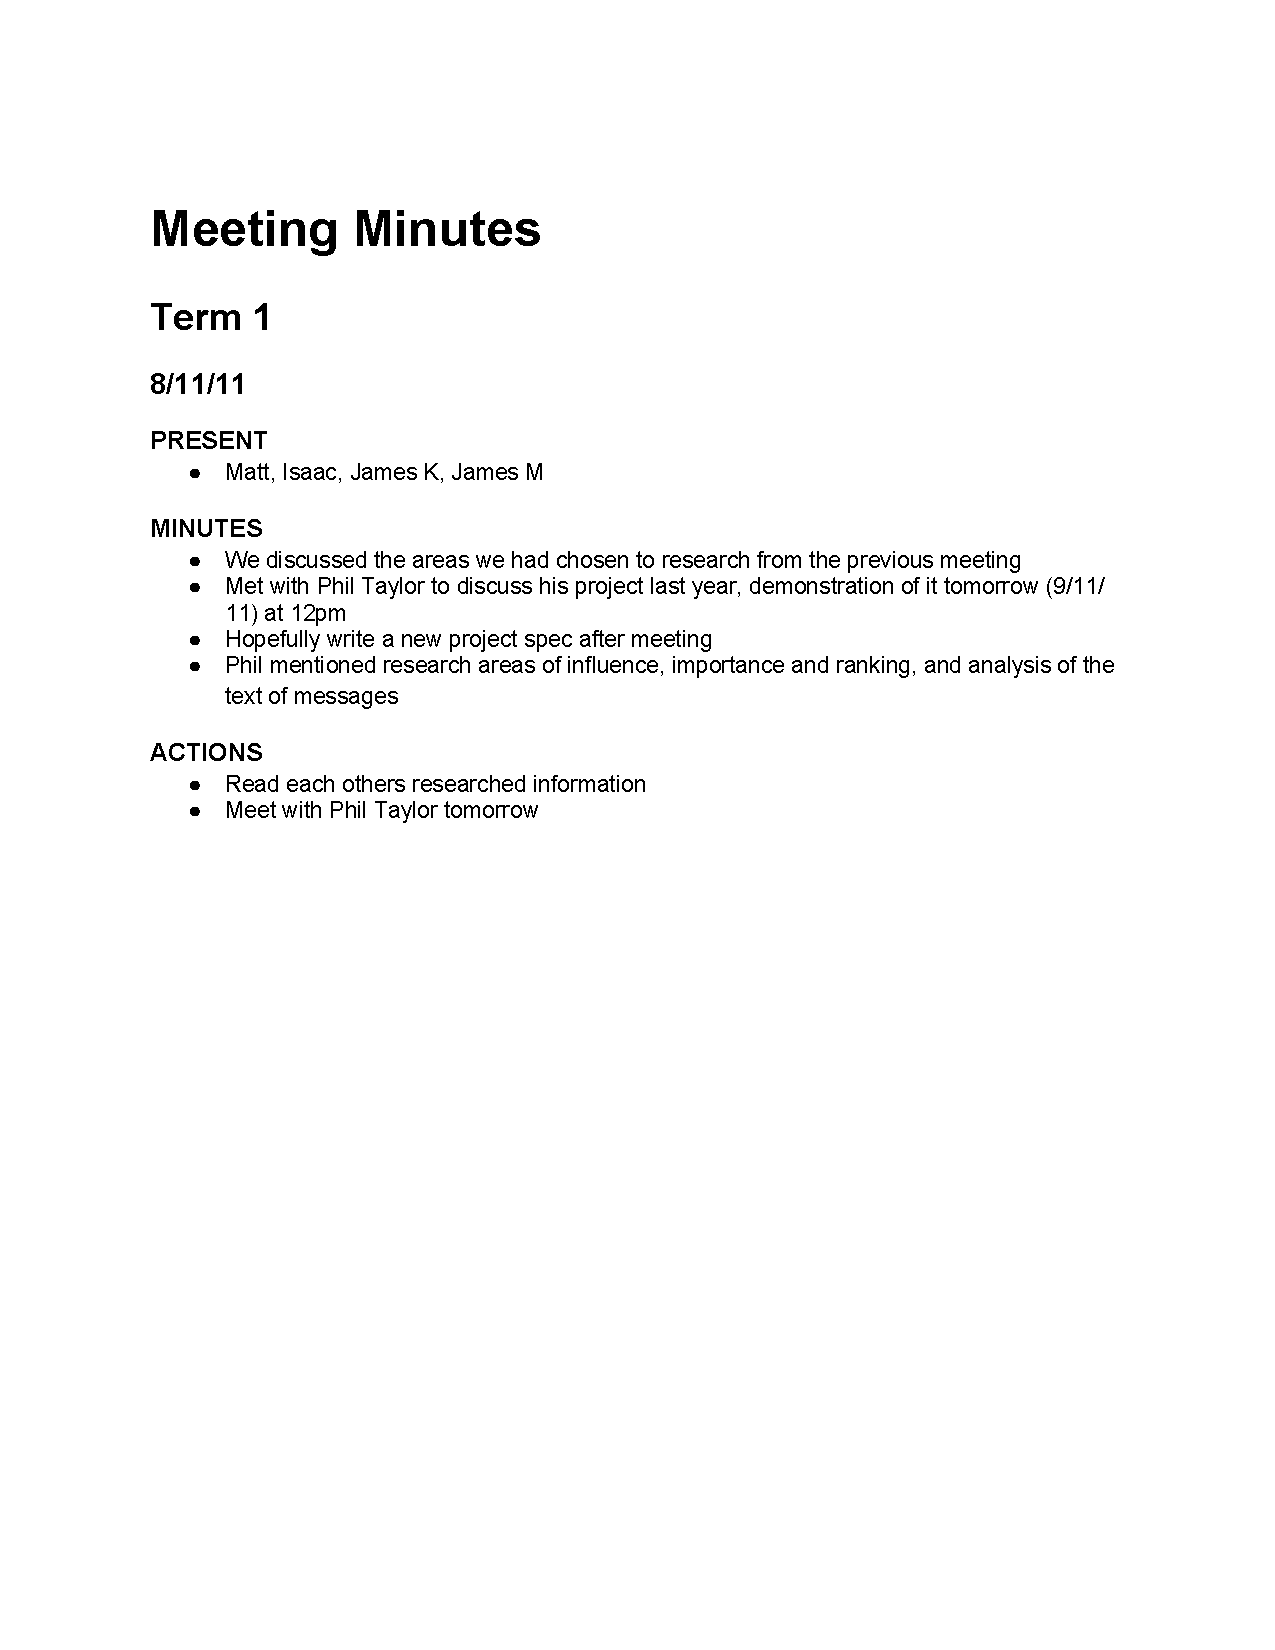
\includepdf[pages=-]{./pdf/minutes}

% End document
\end{document}
